\setauthor{Luna Klatzer}

This chapter will discuss the implementation of the Kipper compiler, detailing its various components, language features, and the thought process behind their development. It will also include comparisons with other languages and provide background information on the design choices made during implementation.

\section{Compiler}
\label{sec:compiler}
\setauthor{Luna Klatzer}

The Kipper Compiler is the core component of the Kipper project, serving as the central piece connecting the Kipper language to its target environment. It functions similarly to other \gls{transpilation}-based compilers, such as the TypeScript compiler, by producing high-level output code from high-level input code—specifically, code written in the Kipper language. The syntax of the language is predefined and implemented using the lexer and parser generated by the \Gls{antlr4} parser generator. 

An interesting aspect of the Kipper compiler is its largely modular design, which allows various components to be replaced or extended as needed. This modularity primarily serves to enable the compiler's structure to adapt to future changes in the language and its target output environment. Given the rapid evolution of web technologies and the frequent addition of new functionality, it is essential to ensure that the compiler remains current. Additionally, this design allows users to create plugins or extensions for the compiler to support custom functionality that may not be natively available.

Furthermore, as discussed in greater detail in Section~\ref{sec:output-generation}, the compiler is capable of targeting more than one output format. Specifically, it supports both standard JavaScript, adhering to the ES6/ES2015 specification, and standard TypeScript as defined by Microsoft. Similar to other compiler systems, users can configure the compiler according to their preferences and specify the desired target language.

\subsection{Stages of compilation}
\setauthor{Luna Klatzer}

The Kipper compiler processes the program through multiple phases, each building upon the previous one to progressively enrich the semantic and logical representation of the program. The phases and their corresponding responsible components are as follows:

\subsubsection{Lexical Analysis}
\begin{itemize}
	\item Detailed explanation in Section~\ref{sec:lexing-parsing}
	\item Performed by: \textbf{Antlr4 Kipper Lexer}
	\item This phase tokenizes the source code into a stream of lexemes, identifying the basic units of syntax.
\end{itemize}

\subsubsection{Syntax Analysis - Parsing}
\begin{itemize}
	\item Detailed explanation in Section~\ref{sec:lexing-parsing}
	\item Performed by: \textbf{Antlr4 Kipper Parser}
	\item In this phase, the lexed tokens are organized into a parse tree based on the grammar rules of the Kipper language.
\end{itemize}

\subsubsection{Parse Tree Translation to AST}
\begin{itemize}
	\item Detailed explanation in Section~\ref{sec:translation-to-the-ast}
	\item Performed by: \textbf{Kipper Core Compiler}
	\item Converts the parse tree into an Abstract Syntax Tree (AST), a more abstract and language-independent representation of the code.
\end{itemize}

\subsubsection{Semantic Analysis}
\begin{itemize}
	\item Detailed explanation in Section~\ref{sec:semantic-analysis}
	\item Performed by: \textbf{Kipper Core Compiler}
	\item This phase is split into three separate steps:
	\begin{enumerate}
		\item Primary Semantic Analysis (see Section~\ref{sec:primary-semantic-analysis}): Validates language semantics such as variable declarations and scope resolution.
		\item Preliminary Type Analysis (see Section~\ref{sec:preliminary-type-analysis}): This phase performs initial type validations and checks. It includes tasks such as loading type definitions that might be referenced elsewhere in the program. These types need to be pre-loaded to ensure they are available and correctly resolved during subsequent stages of compilation.
		\item Primary Type Analysis (see Section~\ref{sec:primary-type-analysis}): Conducts in-depth type validation and resolves type-related issues for the given statements and expressions.
	\end{enumerate}
\end{itemize}

\subsubsection{Target-Specific Requirement Checking}
\begin{itemize}
	\item Addressed shortly in Section~\ref{sec:target-requirements-and-reserved-keywords}
	\item Performed by: \textbf{Target Semantic Analyser}
	\item Ensures compliance with the specific requirements of the target platform (JavaScript or TypeScript). This step is relatively minor and primarily ensures that no code is translated in a way that would cause incompatibilities with the target.
\end{itemize}

\subsubsection{Code Optimization}
\begin{itemize}
	\item Addressed shortly in in Section~\ref{sec:requirements-generation-and-optimizations}
	\item Performed by: \textbf{Kipper Core Compiler}
	\item Performs code optimizations, currently focused on tree-shaking to eliminate unused code.
\end{itemize}

\subsubsection{Target-Specific Translation}
\begin{itemize}
\item Detailed explanation in Section~\ref{sec:output-generation}
\item Performed by: \textbf{Target Translator}
\item Translates the optimized AST into the desired target language (JavaScript or TypeScript).
\end{itemize}

Each phase of the compiler is executed sequentially, with each step requiring the successful completion of the previous one. This ensures that each module of the compiler can safely rely on the correctness and completeness of the information provided by earlier steps. However, this approach limits the compiler's ability to recover from errors or detect all faults in a single execution. As a trade-off, this method simplifies the implementation and reduces overall complexity. Unlike TypeScript, for example, this means that the compiler cannot ignore certain errors and work around them. 

\section{Lexing \& Parsing}
\label{sec:lexing-parsing}
\setauthor{Luna Klatzer}

The first step in the compilation process is the lexing and parsing of the input program. This involves the tokenisation of the program source code, where individual strings are classified into predefined categories, followed by syntactical analysis that organizes these tokens into statements, expressions, and declarations.

In the Kipper compiler, these two steps are carried out by the Kipper Lexer and Parser generated by \Gls{antlr4}, rather than being directly implemented within the compiler itself. These \Gls{antlr4}-generated components are constructed based on the predefined token and syntax rules specific to the Kipper language.

\subsection{Syntax definition}

The primary utility provided by \Gls{antlr4} lies in its ability to generate lexers and parsers automatically from an input file written in the Antlr4-specific ".g4" context-free grammar format. For Kipper, the lexer and parser each have distinct definitions, specifying the individual tokens and the rules for constructing the syntax tree that organizes and groups these tokens.

These definitions are created in a manner similar to other syntactical specification methods, such as BNF (\Gls{backus–naur-form}), commonly used for context-free formal grammars. However, unlike BNF, Antlr4 grammars have the added capability to include programmatic conditions and invocations, enabling more dynamic and adaptable grammar definitions.

\subsubsection{Lexer Grammar Definition}
\label{sec:lexer-grammar-definition}

In the case of the Kipper Lexer, it uses its own token definition file, which defines how characters are grouped into tokens. This file specifies the rules for identifying individual tokens while ignoring special characters that are not required for syntax analysis. Additionally, the lexer separates the matched tokens into various channels, allowing for more efficient handling and categorization during subsequent parsing steps (see Section~\ref{sec:token-channels} for more info).

For example, the lexer grammar includes constructs for identifying both comments and language-specific keywords.

In the grammar as demonstrated in Listing~\ref{lst:kipper-lexer}, comments are directed to a separate channel using the \lstinline|-> channel| annotation. This helps isolate them from the main parsing flow while still retaining them for potential processing or documentation purposes. Pragmas, which are typically compiler directives, are handled similarly but redirected to a \lstinline|PRAGMA| channel.

\begin{lstlisting}[language=antlr4, caption={Sample snippet from the Kipper Lexer grammar}, label={lst:kipper-lexer}]
BlockComment : '/' .? '*/' -> channel(COMMENT) ;

LineComment : '//' CommentContent -> channel(COMMENT) ;

Pragma : '#pragma' CommentContent -> channel(PRAGMA) ;

InstanceOf : 'instanceof';

Const : 'const';

Var : 'var';
\end{lstlisting}

\Gls{antlr4} grammars also include support for defining keywords, operators, and contextual language constructs. For instance, \lstinline|Const| and \lstinline|Var| are tokenized as reserved keywords, ensuring they are recognized unambiguously during lexical analysis. This explicit tokenisation is critical for constructing a clear and predictable syntax tree, which serves as the foundation for the subsequent phases of interpretation and compilation.

\subsubsection{Syntactical Grammar Definition}
\label{sec:parser-grammar-definition}

Like the Kipper Lexer, the Kipper Parser is defined by its own syntax definition file. In this file, various rules are grouped into syntax rules that collectively form a hierarchical structure. The parser traverses this structure to determine which syntactical construct is represented by the individual tokens. These syntax rules are organized in a way that allows the parser to construct a parse tree by following specific paths, with each path representing a distinct syntactical structure in the Kipper language.

For example, a grammar rule defining a function declaration in Kipper could be expressed as seen in Listing~\ref{lst:function-declaration}:

\begin{lstlisting}[float,language=antlr4, caption={Function Declaration Grammar}, label={lst:function-declaration}]
functionDeclaration : 'def' declarator '(' parameterList? ')' '->' typeSpecifierExpression compoundStatement? ;

parameterList : parameterDeclaration (',' parameterDeclaration)* ;

parameterDeclaration : declarator ':' typeSpecifierExpression ;
\end{lstlisting}

In this grammar, the rule for \lstinline|functionDeclaration| begins with the keyword \lstinline|'def'|, followed by a \lstinline|declarator| (which represents the function name or identifier) and then an optional \lstinline|parameterList|. The rule includes a \lstinline|typeSpecifierExpression|, indicating the return type of the function, and optionally a \lstinline|compoundStatement|, which represents the function's body.

The \lstinline|parameterList| rule handles the optional inclusion of one or more parameters, each defined by \lstinline|parameterDeclaration|. Each \lstinline|parameterDeclaration| consists of a \lstinline|declarator| (the parameter's name) followed by a type specification. This structure clearly defines the expected syntax for a function declaration in Kipper, ensuring that the parser can accurately identify and process this construct.

Using these syntax rules, the Kipper parser can build a detailed parse tree, with nodes representing various language constructs, such as function definitions, parameters, and expressions. This hierarchical structure allows for efficient interpretation or compilation of Kipper code.

\subsection{Lexical analysis}

\subsubsection{Primary tokenisation}

The primary task of the lexical analysis is the tokenisation of the individual characters into grouped tokens which represent syntactical elements, such as identifiers, keywords, constant values, etc. Tokens serve as the building blocks for higher-level constructs in the parsing process, providing a simplified and structured representation of the raw source code.

The step of tokenisation is fairly straightforward as it simply follows the definitions provided in the grammar file (see Section~\ref{sec:lexer-grammar-definition}) and throws errors in case no associated token definition is found. Each token is assigned a specific type based on the grammar rules, ensuring that the source code adheres to the language's syntactical structure. If a character sequence does not match any defined rule, an error is raised, indicating the presence of invalid syntax.

The lexer operates as a state machine, scanning through the input character stream and categorizing sequences based on patterns defined in the grammar. These patterns may include regular expressions to match identifiers, numerical constants, or specific language keywords. Once tokens are identified they are put into the associated channels as explained in~\ref{sec:token-channels}.

\begin{figure}[h!]
	\centering
	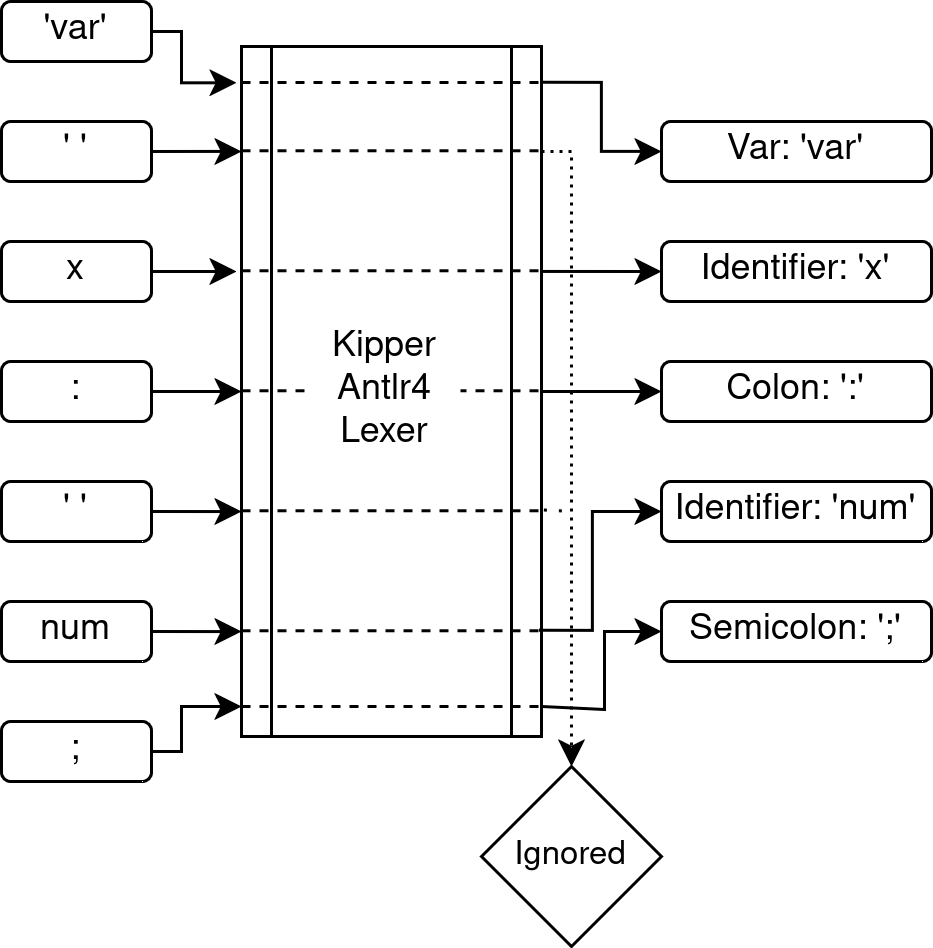
\includegraphics[scale=1]{./pics/Lexer-Algorithm.drawio}
	\caption{The lexing process which categories the various tokens}
	\label{fig:implementation:Lexer-Algorithm}
\end{figure}

\subsubsection{Token Channels}
\label{sec:token-channels}

Next to the definition of the various tokens the grammar file also specifies what channel each token should be put into. These channels act as a stream of tokens where each stream represents different semantic parts of the program.

The channels which are implemented in the case of Kipper are:

\begin{itemize}
	\item \textbf{Default channel}
	\item \textbf{Comments channel}
	\item \textbf{Pragma channel}
	\item \textbf{Ignored channel}
\end{itemize}

The \textbf{default channel} serves as the primary stream, storing nearly all tokens in the program. It is the main channel used during the parsing step to construct a parse tree of the program.

The remaining channels are special-purpose streams that are excluded during parsing and cater to specific functionalities:

\begin{itemize}
	\item The \textbf{comments channel} is dedicated to storing all comments, which are logically irrelevant to the program and do not require parsing or further processing.
	\item The \textbf{pragma channel} contains compiler pragmas—special instructions to the compiler that are processed independently from the standard syntax rules.
	\item The \textbf{ignored channel} is reserved for special characters that are significant only for token differentiation but have no logical relevance to the program, such as spaces. While spaces are critical for separating tokens, like with \lstinline|var x| and \lstinline|varx| they do not contribute to the program's logic and are therefore excluded from parsing.
\end{itemize}
	
\subsubsection{Nested Sub-Lexing}
\label{sec:nested-sub-lexing}

Besides standard sequential processing of the input, the Kipper Lexer also employs a technique called sub-lexing. Sub-lexing involves branching off the main lexing process and invoking a sub-lexer that operates under its own set of rules and guidelines. This specialized lexer handles specific subsets of tokens that require unique processing rules.

Sub-lexing is crucial for Kipper due to features such as templating, where code fragments are embedded within strings. In such cases, the lexer must correctly differentiate between string elements and code atoms (the inserted snippets inside the string). By using a simple push-and-pop mechanism, the lexers can function similarly to a stack, layering processing contexts on top of one another. Each context processes its corresponding string subset, enabling correct parsing of both regular syntax and embedded code within strings. This modular approach ensures cleaner handling of complex tokenisation scenarios and increases the lexer's flexibility.

\begin{figure}[h!]
	\centering
	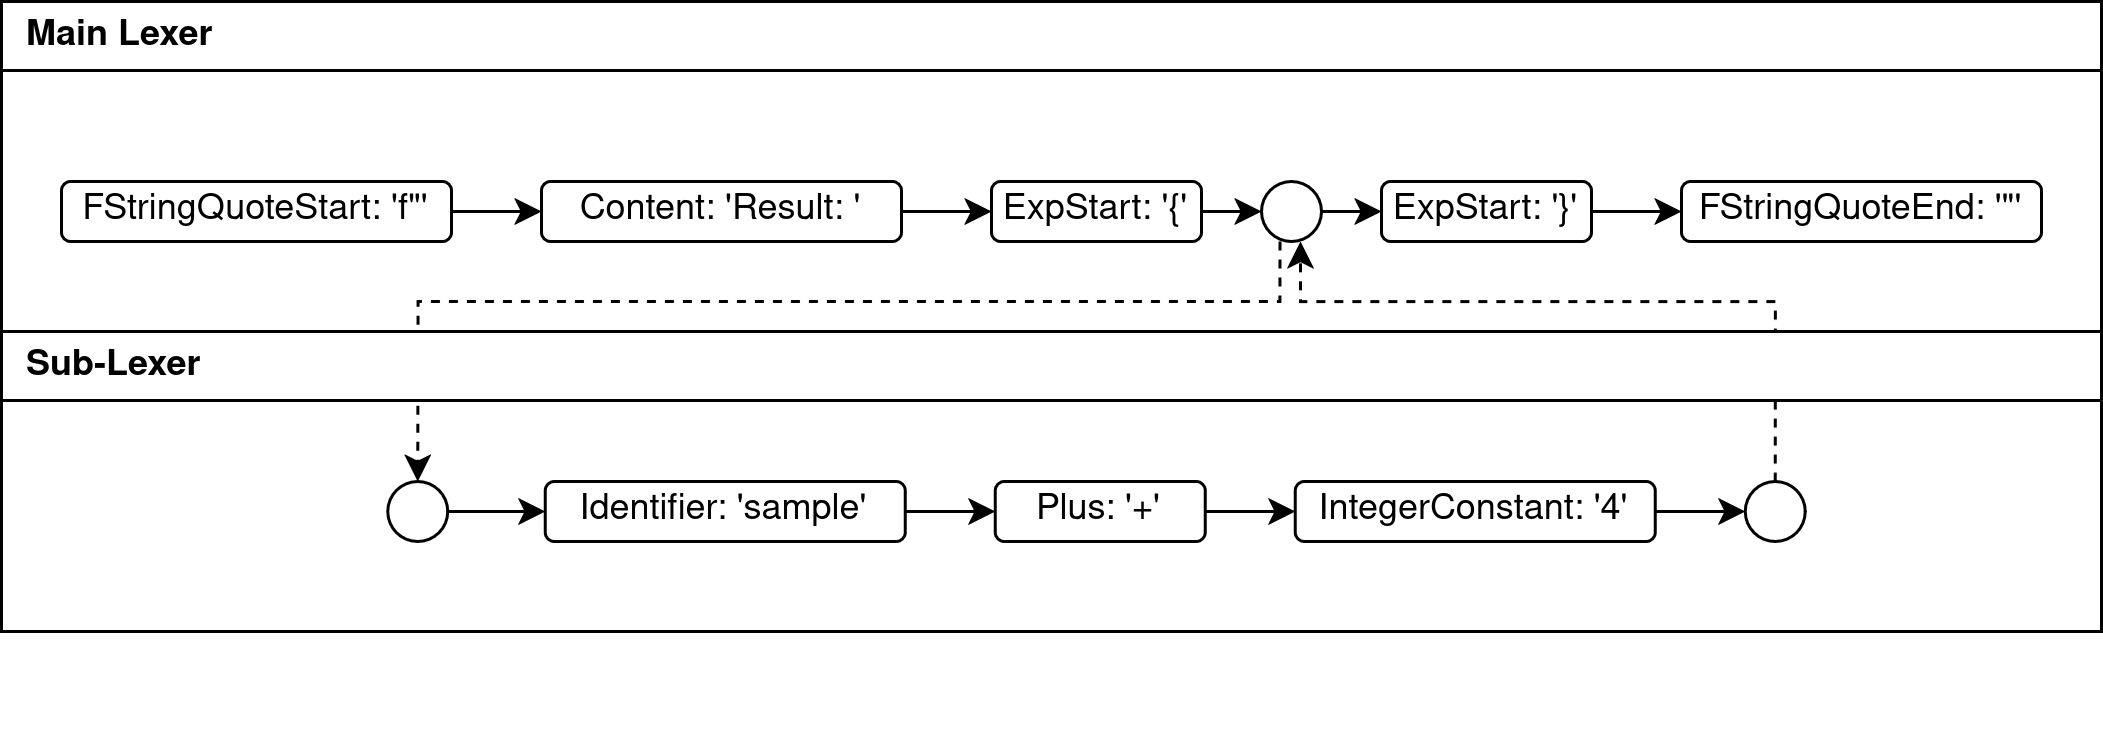
\includegraphics[scale=0.85]{./pics/Sub-Lexer.drawio}
	\caption{The process of invoking a sub-lexer with the sample input \lstinline|f"Result: \{sample + 4\}"| (An example of a template string, or also format string, in the Kipper language), where all content between \lstinline|\{| and \lstinline|\}| is passed onto the sub-lexer.}
	\label{fig:implementation:sub-lexer}
\end{figure}

\subsection{Syntactic analysis}

\subsubsection{Primary syntactic analysis of the token stream}

With the lexer having already identified all tokens in a given program and ensured that only valid elements are present, the parser proceeds to analyse the program's structure and logic. This step is inherently more complex and often demands a significant amount of processing time. The complexity arises partly from the computational effort required to transform a token stream into a viable syntax tree and partly from the design of \Gls{antlr4}, which generates detailed context objects for each node in a program and as such requires a lot of memory and processing to call up each context.

The parser's primary task is to verify that the sequence of tokens conforms to the grammatical rules specified by the Kipper grammar. This involves checking whether constructs such as statements, expressions, and control structures are correctly formed.

\subsubsection{Building the parse tree}

Similar to the hierarchical structure defined by Kipper's grammar rules, the parse tree generated by the Kipper Parser also exhibits a hierarchical organization. Each parse node may have multiple child nodes and is connected to a single parent node, positioned syntactically one level higher within the tree. These nodes can either represent a rule node, such as \lstinline|expression|, or correspond directly to a simple lexer token.

The construction of a parse tree begins with a designated root node representing an entire file. From this root, branching occurs through intermediate rule nodes that capture various grammatical constructs, such as statements, definitions and expressions. These intermediate nodes eventually lead to leaf nodes, which are simple lexer tokens forming the smallest syntactic components of the program, such as identifiers, keywords, operators, and literals.

This hierarchical structure enables easy traversal and analysis of the program during later stages of compilation or interpretation. For instance, an arithmetic expression in a program, such as \lstinline|a + b * c|, would form a sub-tree where the root node corresponds to an expression rule, with child nodes representing the individual terms and operations in the correct precedence order.

A simplified representation of this tree structure is shown in Figure~\ref{fig:implementation:parse-tree}.

\begin{figure}[h!]
	\centering
	\includegraphics[scale=0.95]{./pics/Parse-Tree.drawio}
	\caption{A simplified parse tree representation of the statement \lstinline|var x: num = 4;|.}
	\label{fig:implementation:parse-tree}
\end{figure}

\subsubsection{Programmatic conditions \& context-sensitive rules}

In addition to standard context-free rules, there are grammar rules that incorporate programmatic conditions, requiring specific requirements to be met beyond the standard syntactic structure. These rules are inherently context-sensitive, as they cannot be identified without considering the program’s position and overall logic.

An example of a context-sensitive rule is the compound statement \lstinline|{ }|, which groups multiple statements and is typically used as the body of functions and methods. By definition, such statements are generally permitted only as top-level program nodes or as children of other statements, excluding cases where expressions such as lambda expressions specify one as a child. To accommodate lambdas having a structured body, two types of compound statements are defined. While they serve the same practical purpose, they are logically different due to their different contexts of usage: one as a child of another statement and another as a child of a lambda expression.

\subsection{AST (Abstract Syntax Tree)}
\label{sec:translation-to-the-ast}

The AST represents a tree which groups together the most logically essential elements of a specific items and disregards all the other items not necessary in further processing. Lexer tokens, such as \lstinline|:|, \lstinline|=| or \lstinline|;| may be important syntactically as indicators for specific operations and structures, but once a specific parser rule kind has been determined and the meaning can be derived from that alone these tokens are not necessary anymore and can be discarded.

\subsubsection{Parse Tree Walking}

To transform the parse tree generated by the Kipper Parser, the compiler uses a tree-walking algorithm that systematically traverses the tree by entering and exiting grammar rules. During this process, the algorithm invokes specific handlers when they are defined for particular parse nodes. These handlers are designed to process only the most significant parse nodes, which typically correspond to essential syntactic constructs of the source code.

When a handler is called, it constructs a new AST node and attaches it to the growing AST. This selective processing approach ensures that irrelevant parse tree details, such as redundant intermediate nodes or syntactic artefacts, are automatically excluded from the AST. The resulting AST is a simplified and more abstract representation of the program's structure, capturing only the semantically relevant elements needed for subsequent stages of the compilation process.

The AST generation result of such a tree walk process can be seen in Figure~\ref{fig:implementation:ast}.

\begin{figure}[h!]
	\centering
	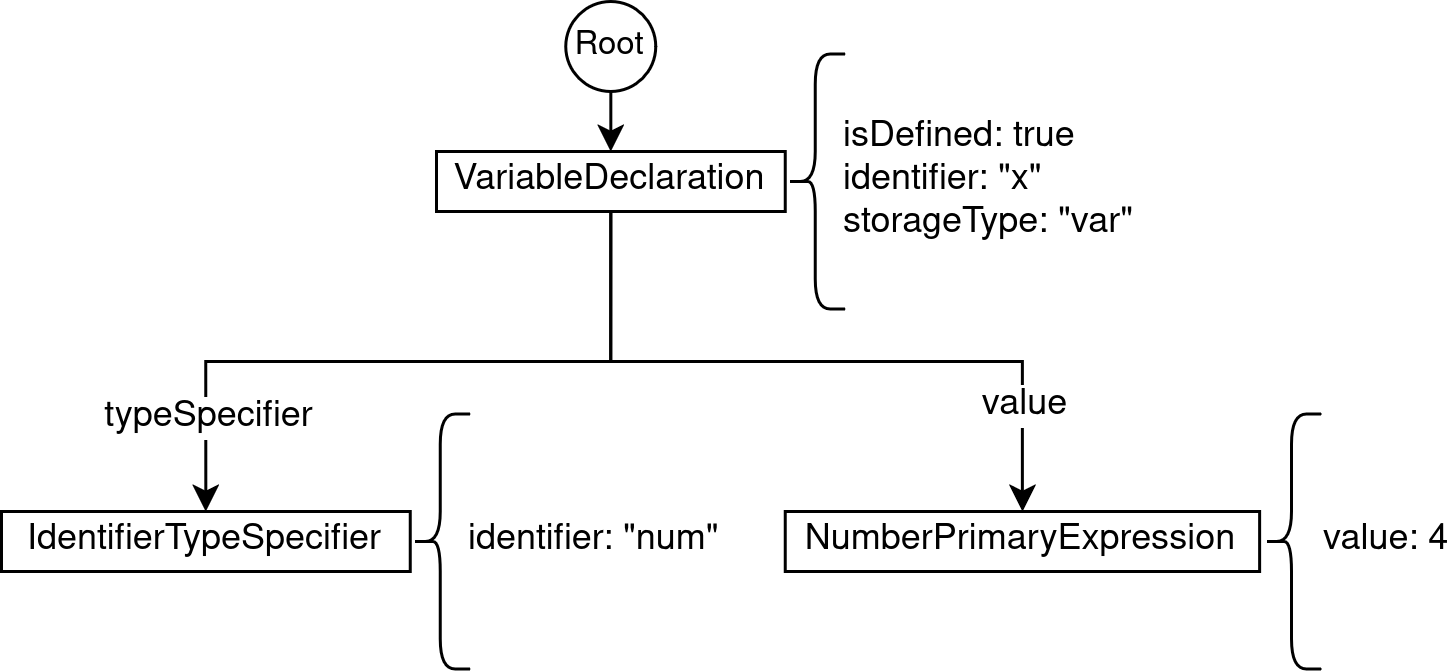
\includegraphics[scale=1]{./pics/AST.drawio}
	\caption{An AST produced by the statement \lstinline|var x: num = 4;|. The data in the brackets is in reality only defined and error checked during semantic analysis (see Section~\ref{sec:semantic-analysis}), but for the sake of clarity it is already provided here as to not cause confusion due to the missing metadata.}
	\label{fig:implementation:ast}
\end{figure}

\subsubsection{Utility provided by the AST}

In addition to providing a simplified abstraction of the original parse tree, individual AST nodes also handle processing for several subsequent stages. Encapsulating these steps within a single class allows semantic analysis and type analysis to be efficiently layered and properly structured. This design is a core aspect of the compiler, as it centralizes data storage and ensures that the results of one processing stage directly influence subsequent stages.

For instance, if a node fails to successfully complete semantic analysis, the subsequent stages are automatically skipped. The node and any related parent structures are marked as faulty, allowing the compiler to handle errors gracefully without immediately crashing (see Section~\ref{sec:error-recovery} for a detailed explanation). Furthermore, the standardized and detailed structure of the AST enables easy integration with other processing steps, as it stores or references all necessary information for specific parts of a program. This is particularly important during output generation (see Section~\ref{sec:output-generation}), where all existing information is required to accurately generate output code which logically adheres to the original program.

\section{Semantic Analysis}
\label{sec:semantic-analysis}
\setauthor{Luna Klatzer}

Semantic analysis is the most complex and critical stage of the compiler, as it extracts essential logical information from the input program and populates the AST built in the previous step with the essential information related to each individual node, ensuring that subsequent processing steps have the necessary data to operate correctly.

Semantic analysis can be broadly divided into two key tasks:

\begin{itemize}
	\item \textbf{Evaluating Semantic Data}
	\item \textbf{Validating Integrity and Raising Errors}
\end{itemize}

These tasks are inherently interdependent, as the compiler typically operates on an assertion-based principle—expecting specific conditions to be met and raising an error when the required input is absent or invalid.

Processing can differ largely in size depending on the node in question, as certain nodes can take advantage of the fact that certain truths are implicitly implied by the parser and therefore don't require verification. Other more ambiguous expressions or statements may require more checks to verify that the input code is valid.

\subsection{Separation of Concerns}
\label{sec:separation-of-concerns}

The Kipper compiler utilises the AST as the foundation for semantic analysis, traversing the tree and analysing individual nodes. This approach follows the principle that each node is responsible for processing itself and its children, allowing nodes to be evaluated independently of their broader context while focusing on their essential aspects. This methodology is particularly significant, as Kipper aims to preserve the abstract program structure and ensure that each node possesses the necessary information for translation. This differs from other compilers, which may employ a flat translation approach, generating symbol tables and instructions as needed without maintaining abstraction.

This design also establishes a trust-based system in which parent nodes can rely on their children to provide the required information for later translation. Each AST node implementation consists of the class itself, an interface defining the semantic data to be populated, and an interface defining the type-related semantic data to be populated. This separation of concerns is a distinctive feature of the Kipper compiler, as semantic and type analysis are often performed concurrently or combined in other compilers. However, in Kipper, the entire AST is traversed separately for each semantic analysis stage.

This staged approach is essential for maintaining program integrity, ensuring logical processing order and guaranteeing that all required data is available when needed. For example, references can bypass the regular processing sequence and may require specific data to be available from another node. To enforce this logic and prevent any logical processing issue or circular reference issue, the Kipper compiler follows a strict rule: each stage must be internally complete and may only reference data generated by earlier nodes in the program or by any node in a preceding stage.

\subsection{Algorithm}

The Kipper compiler performs a total of five distinct steps during semantic analysis, though two of these play a relatively minor role, as they currently apply only to specific use cases. One of these is the warnings check, which is only supported for certain nodes and simply invokes the warning check function if a node has implemented it. The other is more closely related to target generation, as it executes additional semantic checks defined by the specified target (see Section~\ref{sec:target-requirements-and-reserved-keywords} for more info)

The remaining three stages are the most significant, as they each contribute to a specific aspect of semantic analysis, node integrity verification and data definition. These stages are as follows:

\begin{itemize}
	\item \textbf{Primary Semantic Analysis}
	\item \textbf{Preliminary Type Analysis}
	\item \textbf{Primary Type Analysis}
\end{itemize}

Each stage follows the same traversal algorithm, where the compiler begins at the root AST node and recursively invokes checks on its child nodes as demonstrated in Figure~\ref{fig:implementation:semantic-analysis-tree-walking}. These child nodes, in turn, call their own children, continuing the process throughout the tree. This traversal can be described as a bottom-to-top, left-to-right approach in terms of the AST or as a top-down, left-to-right order from the smallest child to the greatest parent when considering a regular file with individual lines.

\begin{figure}[h!]
	\centering
	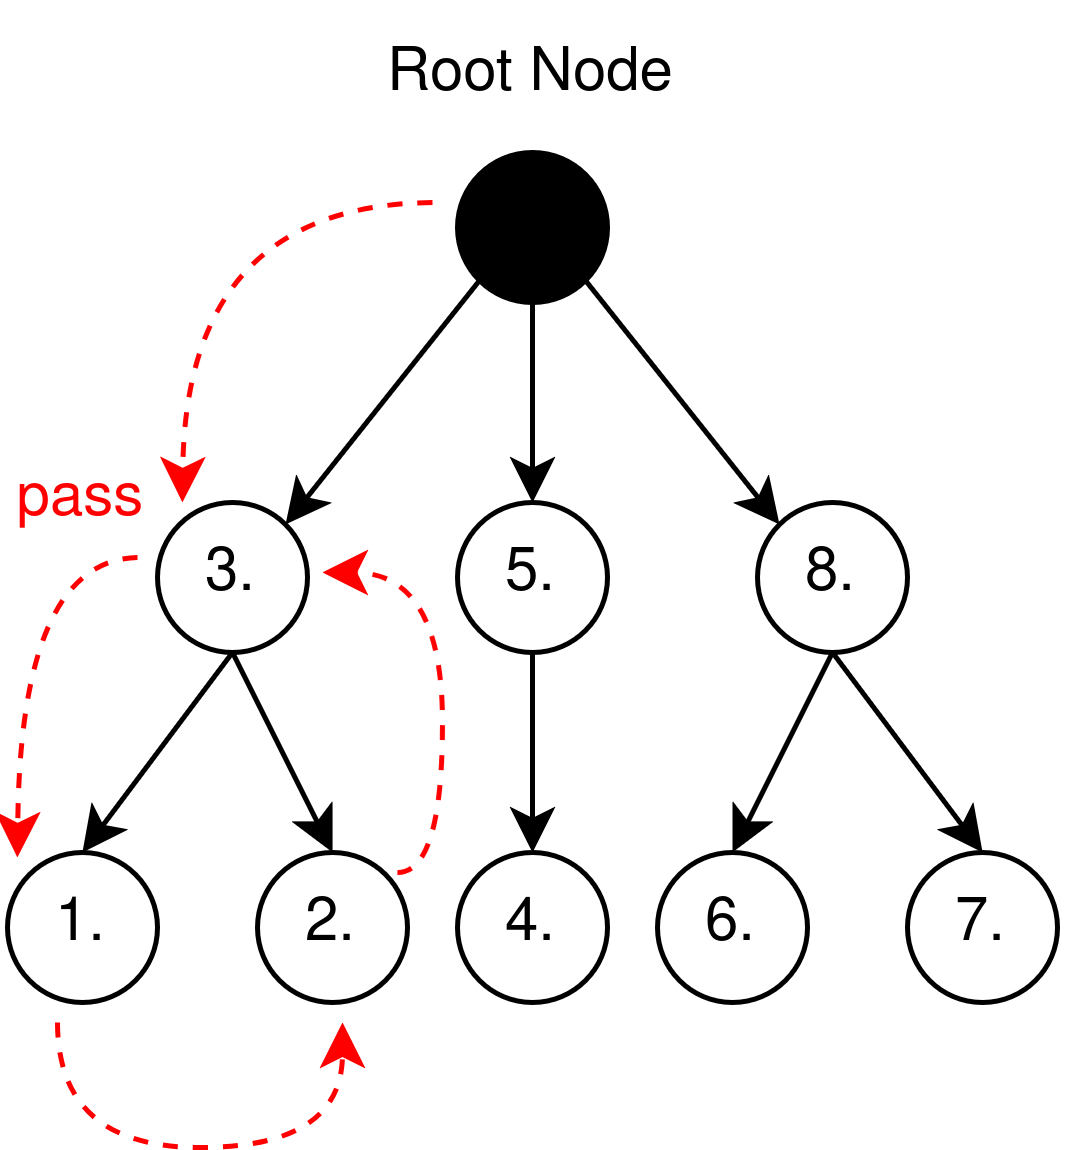
\includegraphics[scale=1]{./pics/Semantic-Analysis-Tree-Walking.drawio}
	\caption{A simplified representation of the semantic analysis tree-walking algorithm. The red dotted line illustrates the path the compiler follows to locate the outermost left leaves, which are processed first, before backtracking to process their parent node. Each node has a ordinal number assigned indicating the order in which it is processed.}
	\label{fig:implementation:semantic-analysis-tree-walking}
\end{figure}

Once a node has completed processing, it will have defined its own semantic data object, storing the necessary information for that specific node. If no data is present, this indicates that the node has failed processing, and an error has already been generated either within that node or in a related child node.

\subsection{Primary Semantic Analysis}
\label{sec:primary-semantic-analysis}

Primary semantic analysis is the initial stage of semantic analysis and is responsible for handling fundamental aspects of a program, such as verifying the availability of names for declarations and definitions, evaluating references, and processing other essential elements. This stage does not involve type checking but instead focuses solely on extracting and validating general semantic data from the core elements of the language. Every node in the AST must undergo this step, as without it, the node would lack all functionality.

This step also is largely responsible for verifying references by building up the symbol tables for the various scopes created by functions, compound statements, classes or other related elements. (see Section~\ref{sec:reference-handling-and-scopes} for further info). 

\subsection{Preliminary Type Analysis}
\label{sec:preliminary-type-analysis}

Preliminary type analysis serves as a precursor to standard type analysis, focusing on processing type definitions before other elements reference or modify them. This step is essential, as types do not always follow a strict hierarchical structure. For instance, a class definition contains elements that reference the class type itself, despite being its children.

This scenario conflicts with the principle outlined in Section~\ref{sec:separation-of-concerns}, which states that a node may only reference elements from previous stages of semantic analysis or nodes already processed before it. Since child nodes must be analysed before their parent nodes, reversing this order would be problematic. To address this, preliminary type analysis ensures that types are loaded first, allowing them to be referenced later without the risk of missing or undefined types. This approach maintains the integrity of the algorithm and preserves the intended order of each semantic analysis stage.

As in the previous stages, this step populates the essential symbol tables with the types defined and processed during this step, and verifies their validity.

\subsection{Primary Type Analysis}
\label{sec:primary-type-analysis}
\setauthor{Luna Klatzer}

Primary type analysis is the final major stage of semantic analysis, responsible for performing type checks, handling type operations, and resolving type references. Given its role in managing the complexity of objects, interfaces, classes, and unions, it serves as a fundamental component of the compiler. Similar to primary semantic analysis, it ensures the correctness of references and verifies that all type references are valid.

During this phase, all nodes have their type data defined, specifying what type information they store and how they function within a given context. In the case of expressions, this means determining the type to which they evaluate, enabling parent nodes to compare child nodes and validate operations, such as arithmetic operations between numerical values. This is crucial for expressions, as they are composed hierarchically, requiring validation of child nodes within their specific context.

In contrast, statements and declarations do not evaluate to a type. While they may perform operations or define types, they cannot be used within another node as part of an expression, except as standalone instructions within a program.

\subsection{Reference Handling and Scopes}
\label{sec:reference-handling-and-scopes}

Reference handling in Kipper operates similarly to most other languages, relying on individual scopes with their own symbol tables that store variables, functions, types, and other relevant entries. These scopes are structured in a hierarchical manner, allowing each scope to access information from the ones below it.

This mechanism is crucial throughout semantic analysis, as each stage is responsible for managing symbol table entries, ensuring that references are valid, and preventing improper overwriting or modification of existing entries.

 \begin{figure}[h!]
	\centering
	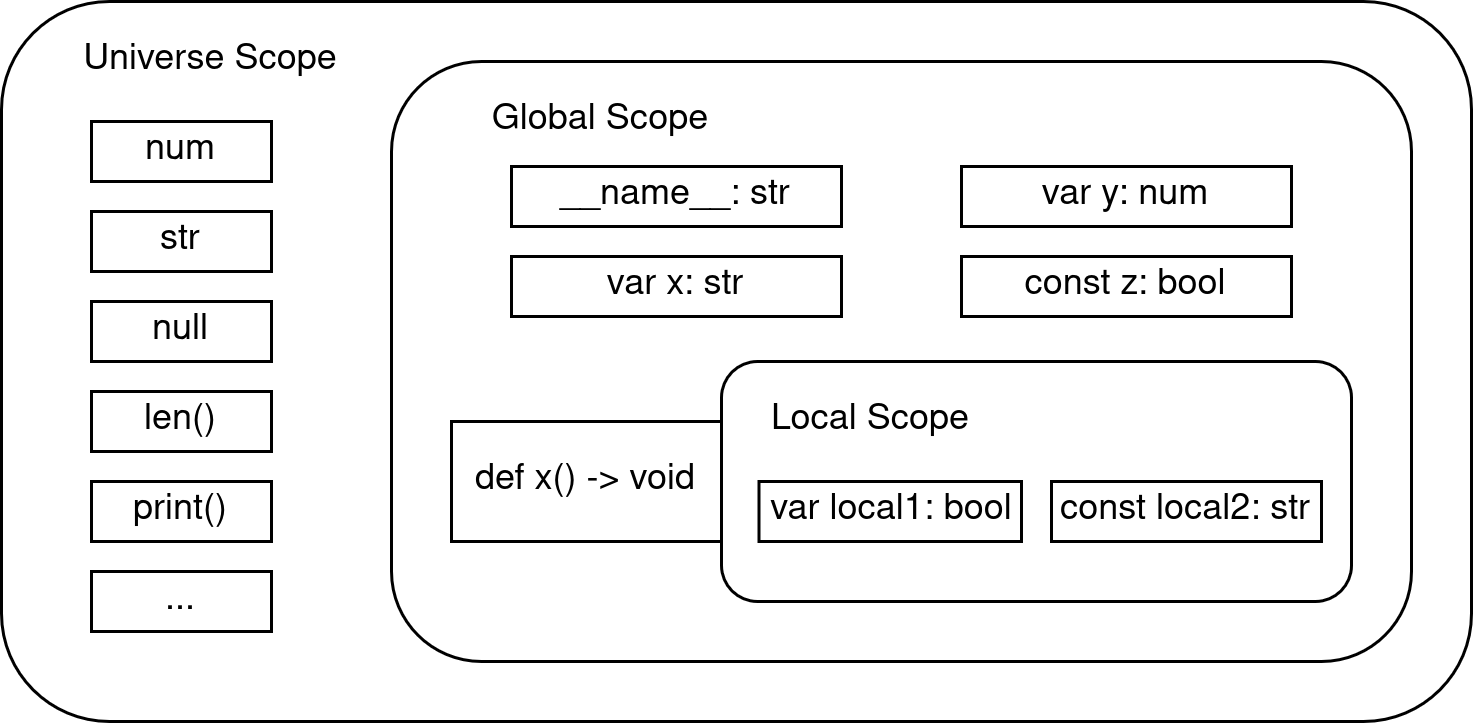
\includegraphics[scale=1]{./pics/Kipper-Scopes.drawio}
	\caption{A simplified representation of the various scopes within Kipper that each act as a layer on top of a stack.}
	\label{fig:implementation:kipper-scopes}
\end{figure}

Kipper currently implements three types of scopes as also visualised in Listing~\ref{fig:implementation:kipper-scopes}:

\begin{itemize}
	\item \textbf{Universe Scope}: This scope defines all built-in types and functions that are always available in Kipper.
	\item \textbf{Global Scope}: This scope contains all global definitions for a specific Kipper program, including file-specific built-ins such as \lstinline|name|, which returns the filename.
	\item \textbf{Local Scope}: Any scope nested within the Global Scope is considered a Local Scope. Entries defined within a Local Scope are accessible only within that scope and its child scopes.
\end{itemize}

Within a Kipper program, only the \textbf{Local Scope} can be defined by the user, while all other scopes are either compiler-bound or file-bound.

\section{Error recovery}
\label{sec:error-recovery}
\setauthor{Luna Klatzer}

The concept of error recovery is fundamental to most modern compilers, as it enables the detection and reporting of multiple errors within a single compilation run. Basic compilers often employ an immediate fail-safe approach, terminating the compilation process upon encountering an error to prevent incorrect assumptions about the program. While this approach preserves the integrity of the compilation process, it presents a significant drawback: in large and complex programs, developers must repeatedly correct errors and recompile to identify additional issues, resulting in inefficient error handling and unnecessary delays during development.

To address these challenges, Kipper implements its own error recovery algorithm, which allows the compiler to recover from errors and continue processing by advancing to subsequent expressions or statements that are not directly associated with the original error node.

However, Kipper's error recovery is limited to the semantic and type analysis phases. The parser, as described in Section~\ref{sec:lexing-parsing}, does not support error recovery and terminates processing upon encountering a syntax error. This behaviour is atypical for a lexer and parser, as they usually allow parsing to continue despite syntactically faulty code blocks. However, due to specific limitations in the version of \Gls{antlr4} used, this functionality is not currently supported.

\section{Output Generation}
\label{sec:output-generation}
\setauthor{Lorenz Holzbauer}

The Kipper compiler is built on a modular architecture, allowing for the definition of custom output targets and providing flexibility to accommodate various use cases. This modularity extends beyond basic configuration, enabling developers to specify target-specific features and behaviours. The modular design is structured around two primary components: the frontend and the backend.

For comparison, the GCC (\Gls{gnu-compiler-collection}) compiler achieves modularity by dividing its architecture into three components, as illustrated in Figure~\ref{fig:implementation:gcccompiler}. The frontend is responsible for verifying syntax and semantics, scanning the input, and performing type checking. It subsequently generates an intermediate representation (IR) of the code.

The middle-end then optimizes this intermediate representation, which is designed to be independent of the CPU target. Examples of middle-end optimizations include dead code elimination and detection of unreachable code. Finally, the backend takes the optimized intermediate code and generates target-dependent code. In the case of GCC, this involves generating assembly code.

\begin{figure}[h!]
	\centering
	\def\stackalignment{r}
	\stackunder{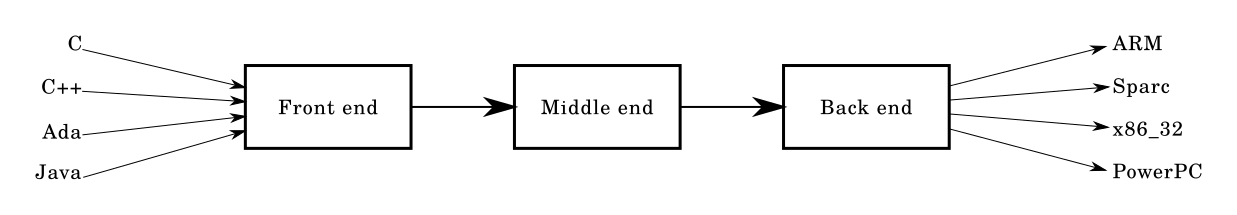
\includegraphics[scale=0.36]{./pics/Compiler_design}}{\scriptsize Source: \href{https://commons.wikimedia.org/wiki/File:Compiler_design.svg}{https://commons.wikimedia.org}}
	\caption{The design of the GCC compiler}
	\label{fig:implementation:gcccompiler}
\end{figure}

As of now, Kipper generates either TypeScript or JavaScript code as its output. The target language is specified in the Kipper CLI utility using the flag --target={js|ts}. If this flag is not provided, the default target is JavaScript.

Currently, Kipper does not include a middle-end component. This decision was made to avoid the additional complexity associated with implementing a full middle-end, as the resulting performance improvements in generated code would be only marginal. Instead, the frontend directly passes the AST (Abstract Syntax Tree) to the backend. While Kipper does perform some post-analysis optimizations, these are presently limited to tree-shaking.

\subsection{Role of the AST in the output generation}

Kipper generally uses an AST as the primary representation of the code from the input program. The AST serves as a hierarchical structure that represents the program's source code. The root node of the AST corresponds to the entire program, while each child node represents a specific construct such as a statement, scope, or other language feature.

Each node in the AST contains the semantic data and type-related information of the corresponding statement, as well as a string representation of the original parser node. Additionally, every node includes a kind identification property—a unique, hard-coded number in the compiler—to uniquely identify the type of the node. This property aids in determining the type of construct, such as a declaration, an expression, or a statement.

Every node also maintains a list of child nodes, representing nested or dependent components of the construct. Once the AST is fully constructed, it is wrapped and passed to the code generator for further processing.

\subsection{Algorithms used for Output Generation}

There is a plethora of algorithms available to generate code in the target language. They can be classified by their input data structure. Some algorithms need a tree-like IR (\Gls{intermediate-representation}), others need a linear IR structure.

\subsubsection{Linear Algorithms}

Linear algorithms are commonly employed when compiling high-level languages to machine code or bytecode. These algorithms treat the input as a flat, ordered sequence and process it sequentially. Intermediate representations (IR) are typically in the form of three-address code or static-single-assignment (SSA) form. Linear algorithms process the code one instruction at a time in sequence. Upon completion of an instruction, it is added to a list, which is eventually concatenated and written to the output file.

Three-address code consists of three operands and typically represents an assignment with a binary operator~\cite{wiki:threeaddress}. An instruction may have up to three operands, although fewer can also be used. In Listing~\ref{lst:implementation:threeaddresscode}, the problem is divided into multiple instructions. This structure allows the compiler to easily translate the instructions into assembly language or bytecode, which share a similar format. Additionally, the compiler can identify unused code by determining whether a variable is referenced later in the code.

\begin{lstlisting}[float,language=TypeScript,caption=Three-address code,label=lst:implementation:threeaddresscode]
// Problem
x = (-b + sqrt(b^2 - 4*a*c)) / (2*a)

// Solution
t1 := b * b
t2 := 4 * a
t3 := t2 * c
t4 := t1 - t3
t5 := sqrt(t4)
t6 := 0 - b
t7 := t5 + t6
t8 := 2 * a
t9 := t7 / t8
x := t9
\end{lstlisting}

The Static Single-Assignment (SSA) form is an alternative intermediate representation in which each variable is assigned exactly once~\cite{wiki:singlestatic}. It is widely used in compilers such as GCC. The primary advantage of SSA is that it simplifies the code and enhances the effectiveness of compiler optimizations.

In Listing~\ref{lst:implementation:staticsingleassignmentform}, a variable \lstinline|y| is assigned twice. The first assignment is redundant. In SSA form, the compiler can identify that the assignment to \lstinline|y1| is unnecessary, as it is not used in the subsequent code. Optimizations improved by the use of SSA include dead-code elimination, constant propagation, and register allocation.

\begin{lstlisting}[language=TypeScript,caption=Static single-assignment form,label=lst:implementation:staticsingleassignmentform]
// Problem
y := 1
y := 2
x := y

// Solution
y1 := 1
y2 := 2
x1 := y2
\end{lstlisting}

\subsubsection{Tree-based Algorithms}

Tree-based algorithms are widely used in \gls{transpiler}s because they preserve the readability and structural integrity of the source code. By maintaining the original scopes and statements, they ensure that the transformed code remains as close as possible to its initial form. To achieve this, code components are stored as nodes in a tree-like structure.

Kipper employs a bottom-up code generation algorithm, in which a tree-walker recursively traverses the syntax tree, starting from the deepest nested nodes to generate the output. This approach was selected for its simplicity in visualization and implementation, as well as its ability to maintain human-readable and easily extendable source code without aggressive transformations. Linear algorithms, by contrast, convert code into intermediate representations such as three-address code or static single-assignment (SSA) form, often stripping away valuable structural and contextual information.

Although tree-based code generation can produce bytecode, which is subsequently optimized and compiled using linear algorithms, it has inherent limitations. Specifically, optimizations remain localized to individual nodes, and the recursive traversal can lead to high computational costs for complex inputs. Due to these constraints, tree-based designs are rarely used in professional bytecode-generating compilers. However, GCC incorporates a tree-based design in two of its language-independent intermediate representations (IRs): GIMPLE and GENERIC~\cite{gcc:gimpletuples}.

\subsection{Generation Algorithm}

The output generation process in Kipper starts by initializing the target environment and setting up any necessary dependencies, as outlined in Section~\ref{sec:requirements-generation-and-optimizations}. Once this setup is complete, the compiler iterates through the previously generated AST nodes, invoking the \lstinline|translateCtxAndChildren| function for each node. This function performs a recursive traversal of the syntax tree, generating code for each child node. Each node returns a string containing its corresponding output code, which is then processed by its parent node. The process continues until the root node collects and merges all generated strings, passing the final output to a function responsible for writing the translated code to a file.

This bottom-up processing approach ensures that child nodes are translated before their parent nodes, allowing parent nodes to retrieve and incorporate necessary information from their children. This methodology is particularly crucial for handling complex structures, as these often rely on the embedded code produced by their child nodes. The generated code is passed up the tree as an array of tokens representing the textual form of the output.

The output generation process ensures reliability by leveraging the fact that the AST has already been validated for syntactic and semantic correctness during earlier compilation phases.

The implementation of this translation algorithm is illustrated in Figure~\ref{fig:implementation:translationalgorithm}.

\begin{figure}[h!]
	\centering
	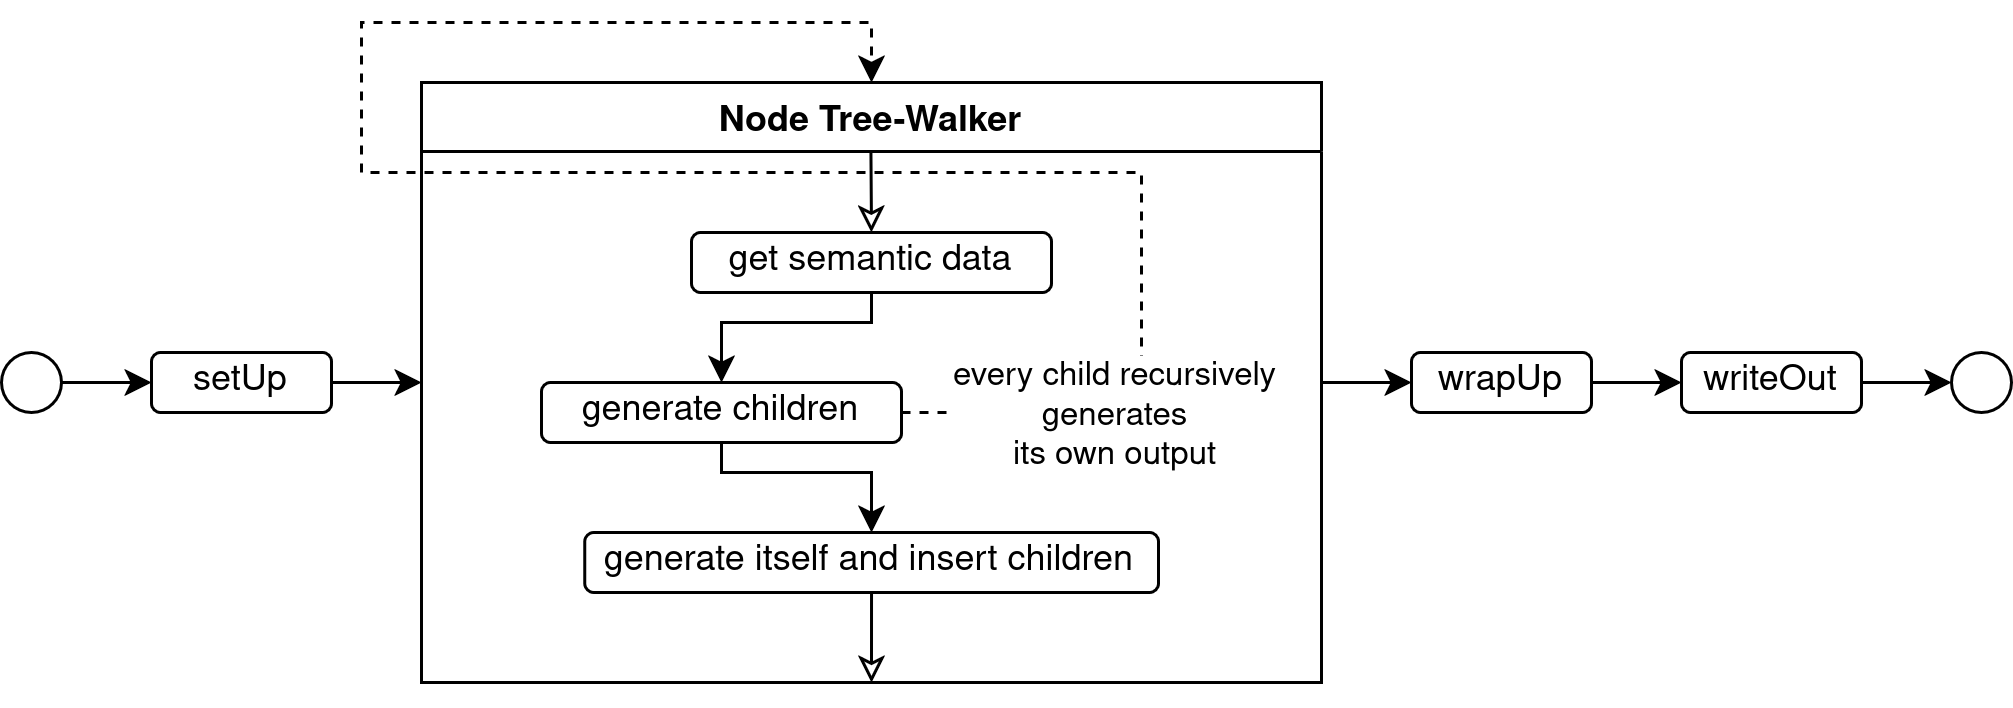
\includegraphics[scale=0.9]{./pics/Output-Generation.drawio}
	\caption{A simplified version of the tree-walker generation algorithm.}
	\label{fig:implementation:translationalgorithm}
\end{figure}

The code generation function of a node accepts the node as an argument and extracts its semantic and type-semantic data. This data is then utilized to translate the node's children—properties defined within the semantic data—into source code. The resulting code fragments are collected into a string array, concatenated, and returned as the final output for that node.

This approach ensures that each node is processed in a structured manner, maintaining consistency in code generation. Listing~\ref{lst:implementation:instanceofgeneration} demonstrates this process with an example of translating an \lstinline|instanceOf| expression, illustrating how the compiler systematically generates code based on semantic analysis.

\begin{lstlisting}[language=TypeScript,caption=The code generation function of a \lstinline|instanceOf| expression,label=lst:implementation:instanceofgeneration]
instanceOfExpression = async (node: InstanceOfExpression): ... => {
	const semanticData = node.getSemanticData();
	const typeData = node.getTypeSemanticData();
	const operand = await semanticData.operand.translateCtxAndChildren();
	const classType = TargetJS.getRuntimeType(typeData.classType);

	return [...operand, " ", "instanceof", " ", classType];
};
\end{lstlisting}

The code generator functions for the individual nodes are implemented in the code generator class \lstinline|JavaScriptTargetCodeGenerator|. Due to the similarity between TypeScript and JavaScript, the TypeScript code generator extends the JavaScript code generator and overrides the functions that are unique to TypeScript. This eliminates duplicate code fragments.

\subsection{Differences between the Target Languages}

The implementation of a compiler or \gls{transpiler} targeting multiple programming languages often requires addressing the specific quirks and requirements of each target. As Kipper is a web development language, it targets both TypeScript and JavaScript. Although both languages share a common foundation, they diverge significantly in their syntax rules, semantics, and type systems.

One of the primary challenges in supporting both JavaScript and TypeScript as target languages lies in their differing treatment of identifiers, reserved keywords, and type declarations. While JavaScript is dynamically typed and relatively permissive regarding variable naming and usage, TypeScript enforces a stricter set of rules due to its static type-checking capabilities.

\subsubsection{Target Requirements \& Reserved Keywords}
\label{sec:target-requirements-and-reserved-keywords}

Both JavaScript and TypeScript have a set of reserved keywords that cannot be used as identifiers. However, TypeScript introduces additional constraints by reserving type-related keywords, which are not present in JavaScript. For example, \lstinline|class| is a reserved keyword in both languages and cannot be used as a variable name. In contrast, TypeScript also reserves names such as \lstinline|let|, \lstinline|number|, and other type names, making them invalid as variable or function names.

Kipper addresses these reserved keywords by checking for them at compile time. The compiler compares the identifiers against a hard-coded list of keywords, and if a match is found, it throws a \lstinline|ReservedIdentifierOverwriteError|. This list includes both the reserved words of JavaScript and TypeScript, which helps minimise redundancy and complexity. Furthermore, this approach encourages the use of sensible variable names, as JavaScript is relatively lenient regarding reserved keywords, as can be seen illustrated in Listing~\ref{lst:implementation:reservedkeywords}.

\begin{lstlisting}[float,language=TypeScript,caption=Reserved Keywords in TS and JS,label=lst:implementation:reservedkeywords]
	// Invalid in TypeScript
	let let = 5;  // Error: Cannot use 'let' as an identifier
	let number = 10;  // Error: Cannot use 'number' as an identifier
	
	// Valid in JavaScript
	var let = 5;  // No error
	var number = 10;  // No error
\end{lstlisting}

\subsubsection{Type Annotations}

TypeScript introduces type annotations as part of its static type system. This means that while generating the TypeScript output, Kipper has to append type information in variable assignments, functions and lambdas. This works by overriding the JavaScript implementation of the code generator function and converting the AST-internal type of the node to a TypeScript type. 

Figures~\ref{fig:implementation:kipper-to-javascript-translation-example} and~\ref{fig:implementation:kipper-to-typescript-translation-example} shows the difference between the JavaScript code generator function and the TypeScript code generator function for variable assignments with the source example \lstinline|var x: num = 5;| being translated. In the code block that generates TypeScript, there are additional code tokens after the storage and the identifier that insert the type of the object into the output code.

\begin{figure}[h!]
	\centering
	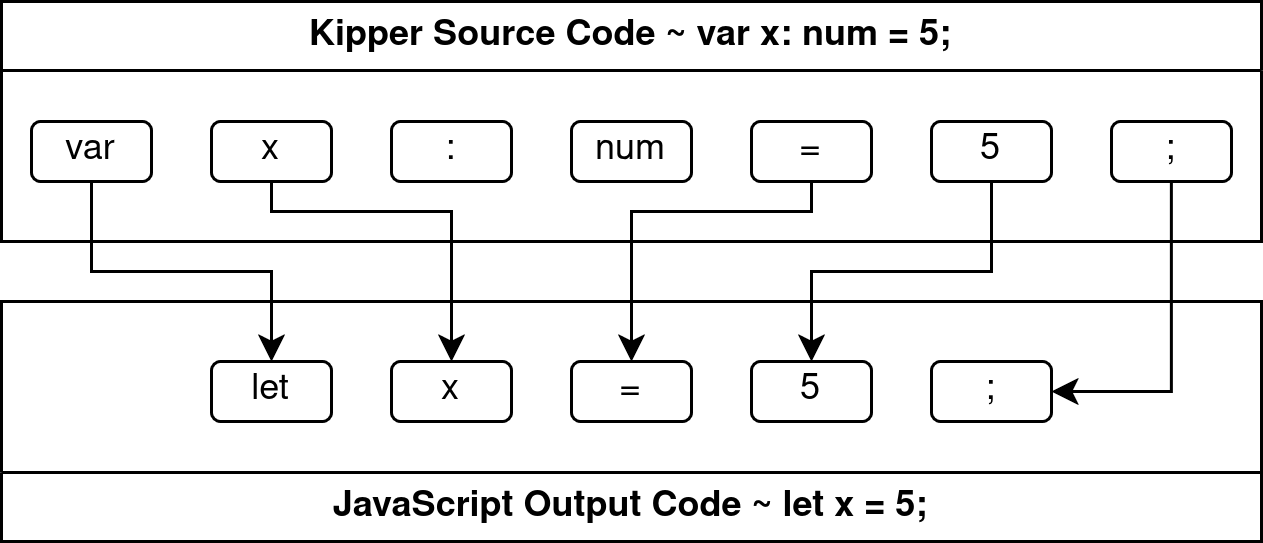
\includegraphics[scale=1.1]{./pics/Kipper-to-JavaScript-Translation-Example}
	\caption{The simplified translation process of the example \lstinline|var x: num = 5;| into JavaScript.}
	\label{fig:implementation:kipper-to-javascript-translation-example}
\end{figure}

\begin{figure}[h!]
	\centering
	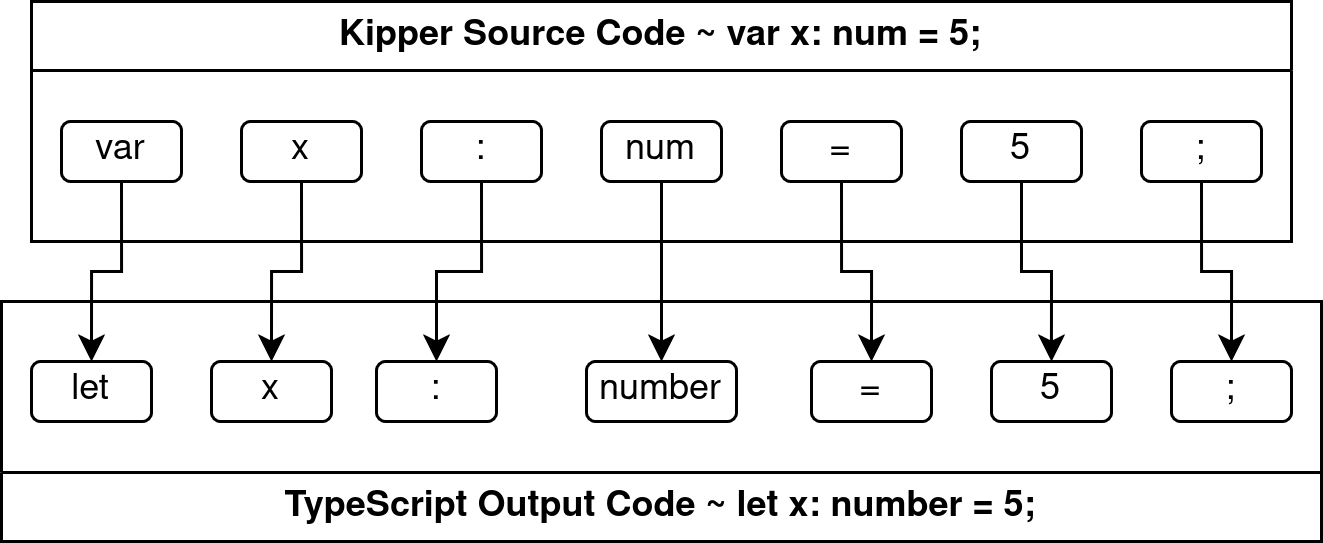
\includegraphics[scale=1.1]{./pics/Kipper-to-TypeScript-Translation-Example}
	\caption{The simplified translation process of the example \lstinline|var x: num = 5;| into TypeScript.}
	\label{fig:implementation:kipper-to-typescript-translation-example}
\end{figure}

Other code generators such as the ones for function declarations and lambdas behave similarly when taking type annotations into account.

\subsection{Target Requirements Generation \& Optimizations}
\label{sec:requirements-generation-and-optimizations}

Kipper is designed to maintain a minimal runtime while ensuring all necessary functionality is included. This requires the compiler to incorporate only the functions and objects essential to the user's program. This approach aligns with the objective of keeping the compiler both modular and lightweight. By eliminating unused components through a process known as "tree-shaking," the resulting output code remains compact and efficient.

Kipper provides a range of built-in functions and features to support its runtime environment. These built-ins are structured using a scoped approach. The global scope includes core runtime features that are always required, such as fundamental type handling and error reporting. Beyond the global scope, additional features—such as helper functions specific to certain syntax, including \lstinline|slice| and \lstinline|match|—are selectively incorporated based on the specific requirements of the compiled program.

\subsubsection{Conditional features}
\label{sec:conditional-features}

Conditional features are runtime components that are included only when explicitly required by the program being compiled. These features range from commonly used operations, such as \lstinline|match| and \lstinline|slice|, to more specialised or program-specific utilities.

Unlike essential runtime components contained within the global scope, conditional features are selectively incorporated based on an analysis of the program's structure and functionality. The inclusion of these features is determined during the requirements generation phase.

As the compiler traverses the AST, it analyses each node to determine whether a specific built-in function or runtime operation is invoked. If a feature such as \lstinline|slice| is detected in the source code, it is marked as necessary and added to the consolidated requirements list. This approach ensures that only the relevant components are integrated into the final runtime environment.

An example of a conditional feature is the \lstinline|slice| function, as demonstrated in Listing~\ref{lst:implementation:slicefunction}.

\begin{lstlisting}[language=TypeScript,caption=The Slice operator being used on a string,label=lst:implementation:slicefunction]
var valid: str = "321";
print(valid[1:2]); // 2
\end{lstlisting}

This function takes an array as input and extracts a section starting from the index specified by the first argument and ending at the index specified by the second argument.

When the compiler encounters the slice operator, it registers the function as necessary within the context of the program being compiled. The code generator called after the semantic analysis then includes it in the output code. This code generator for the example \lstinline|slice| is demonstrated in Listing~\ref{lst:implementation:sliceinternal}.

The compiler calls the slice function in the \lstinline|BuiltInGenerator|. The abstract \lstinline|BuiltInGenerator| class is a collection of functions responsible for generating the code for the built-in functions in a specific target language. This means that each target language must have an individual implementation for each built-in function of Kipper within its output generator, which subsequently adds the corresponding code into the resulting program.

The generator as demonstrated in Listing~\ref{lst:implementation:sliceinternal} generates the required JavaScript code for the function by utilizing the built-in \lstinline|slice| function provided by standard JavaScript.

\begin{lstlisting}[language=TypeScript,caption=Slice in the JavaScript BuiltInGenerator,label=lst:implementation:sliceinternal]
async slice(funcSpec: InternalFunction): Promise<Array<TranslatedCodeLine>> {
	const signature = getJSFunctionSignature(funcSpec);
	const objLikeIdentifier = signature.params[0];
	const startIdentifier = signature.params[1];
	const endIdentifier = signature.params[2];

	return genJSFunction(
		signature,
		`{ return ${objLikeIdentifier} ? ${objLikeIdentifier}.slice(${startIdentifier}, ${endIdentifier}) : ${objLikeIdentifier}; }`,
	);
  }
\end{lstlisting}

The \lstinline|slice| function generated by the code generator as shown in Listing~\ref{lst:implementation:sliceinternal} is represented in Listing~\ref{lst:implementation:slicegenerated}. This function will be executed at runtime and perform the required operation, in this case slicing the given argument.

\begin{lstlisting}[language=TypeScript,caption=Slice in the target language TypeScript,label=lst:implementation:slicegenerated]
slice: function slice<T>(objLike: T, start: number | undefined, end: number | undefined): T {
	return objLike ? objLike.slice(start, end) : objLike;
},
\end{lstlisting}

\subsubsection{The global scope}

The global scope in programming represents the top-level execution context where variables, functions, and objects are accessible throughout the entire runtime environment unless explicitly restricted. In JavaScript, the global scope is particularly significant, as it varies across different runtime environments, such as browsers, Node.js, and Web Workers. This variability necessitates robust mechanisms for identifying and managing the global context to ensure compatibility across environments.

For example, JavaScript defines several global objects, such as \lstinline|window| in browsers, \lstinline|global| in Node.js, and \lstinline|self| in Web Workers. Modern JavaScript unifies these under \lstinline|__globalScope|, a standardized global object that provides a consistent way to access the global scope regardless of the environment. However, not all environments support \lstinline|__globalScope|, which is why fallback mechanisms are often employed.

The Kipper global scope encompasses all the required runtime features. It is crucial that the global scope exists only once, which is why the program checks at runtime whether the scope has already been defined. This logic is demonstrated in Listing~\ref{lst:implementation:globalscopelogic}. The program first checks if \lstinline|__globalScope| is defined and uses it if available. If not, it attempts to use \lstinline|globalThis|, the modern standard JavaScript global object. If \lstinline|globalThis| is not defined, it checks for \lstinline|window| in browser environments, \lstinline|global| in Node.js, or \lstinline|self| in Web Workers. If none of these are defined, it falls back to an empty object. This approach ensures that the \lstinline|__globalScope| variable is always initialised, regardless of the environment, thereby enabling consistent and safe access to the global scope.

\begin{lstlisting}[language=TypeScript,caption=Global Scope Logic,label=lst:implementation:globalscopelogic]
var __globalScope = typeof __globalScope !== "undefined" ? __globalScope :
    typeof globalThis !== "undefined" ? globalThis :
    typeof window !== "undefined" ? window :
    typeof global !== "undefined" ? global :
    typeof self !== "undefined" ? self : {};
\end{lstlisting}

\subsubsection{Internal functions}

Internal functions in Kipper serve as a crucial part of the runtime, but are designed to remain hidden from the user-facing API. These functions provide support for various runtime operations and compiler processes, but are not directly accessible or callable within the user's program. This approach ensures that the runtime environment remains clean and minimal while still delivering the necessary functionality.

An example of an internal function is the \lstinline|assignTypeMeta| function, which adds metadata to a runtime type. This function is essential for runtime type comparison, as discussed in detail in Section~\ref{sec:builtintypes}. Although this function is never exposed to the user, it is invoked internally when for example an interface or array is declared.

A key characteristic of internal functions is their dynamic inclusion in the runtime environment, as also previously discussed in Section~\ref{sec:conditional-features}. During the requirements generation phase, the compiler determines whether any internal mechanisms are required based on the program's functionality. If so, the corresponding internal functions are incorporated into the runtime.

\subsection{Stylistic Choices}

The syntax of Kipper is specifically designed to ease the transition of existing TypeScript and JavaScript developers to Kipper. Consequently, it was important to maintain output that closely resembles these languages as much as possible. This objective was achieved by adhering to the following principles:

\subsubsection{Human Readable Output}

The primary goal of Kipper's output generation is to produce code that mirrors human-written TypeScript or JavaScript as closely as possible. To achieve this, Kipper avoids unnecessary abstractions or layers that could obscure the intent of the code. For instance, variable names and function identifiers are preserved during \gls{transpilation}, without introducing machine-generated names or hashing schemes. This contrasts with languages like CoffeeScript, where the output, although functional, often requires familiarity with the \gls{transpiler}'s conventions to interpret effectively.

\subsubsection{No Code Compression}

Kipper explicitly avoids code compression techniques, such as minification or inlining, which can hinder readability. While compression is useful in production environments to reduce payload size, it is opposed to the goals of Kipper, as it negatively impacts code readability.

\subsubsection{Standardized Style Format}

Kipper enforces a standardized style format for its output to ensure consistency and predictability. It uses two spaces for block-level indentation to maintain clarity and avoid confusion with tab-based formatting. Braces are explicitly used for block delimiters, and semicolons terminate statements, adhering to common TypeScript/JavaScript conventions.

\subsubsection{Scope Visibility}

A critical aspect of Kipper's design is the clear representation of scopes in the generated output. Kipper employs explicit declaration keywords such as \lstinline|let|, \lstinline|const|, and \lstinline|function| to discriminate between variable and function scopes. Indentation and brace placement further enhance the visual hierarchy, making it easy to identify nested scopes and understand their boundaries. This approach contrasts with languages like Python, where indentation alone determines scope, or languages like Lua, where scope visibility may rely on implicit conventions.

\subsubsection{Editable Code}

One of Kipper's unique selling points is that its \gls{transpile}d output is not only readable but also editable. Developers can treat the generated TypeScript/JavaScript code as if it were written manually, enabling seamless integration with existing projects. By making the output editable, Kipper empowers developers to tailor the \gls{transpile}d code to their specific needs without relying solely on the original Kipper source.

\subsubsection{Comparison with Other Languages}

CoffeeScript aimed to simplify JavaScript syntax but often produced output that was hard to debug due to its reliance on non-standard conventions. Kipper avoids these pitfalls by aligning its syntax and output with established TypeScript/JavaScript practices. While TypeScript generates clean and maintainable JavaScript, it requires a compilation step that may introduce additional complexity. Kipper simplifies this process by directly transpiling to both TypeScript and JavaScript, offering flexibility without sacrificing readability. 

Babel, one of the most widely used JavaScript-to-JavaScript \gls{transpiler}s, produces highly optimized output for compatibility across different environments. However, this optimization can result in dense and less human-readable code, making manual modifications more challenging. In contrast, Kipper prioritises maintainability over aggressive optimization, ensuring that the output remains clear, editable, and approachable for developers.

\section{Integrated Runtime}
\label{sec:integrated-runtime}
\setauthor{Lorenz Holzbauer}

\subsection{Runtime Type implementations in other languages}
\label{sec:runtime-other-languages}

\subsubsection{Nominal Type Systems}

Nominal type systems are used in most modern object-orientated programming languages like Java and C\#. In these systems, types are identified by their unique names and can only be assigned to themselves. Additionally, two types are considered compatible, if one type is a subtype of the other one, as can bee seen in Listing~\ref{lst:implementation:javanominaltyping}. Here a  \lstinline|Programmer| is an \lstinline|Employee|, but not the other way around. This means \lstinline|Programmer| instances have all the properties and methods an \lstinline|Employee| has while also having additional ones specific to \lstinline|Programmer|. The relationships are as such inherited, so \lstinline|SeniorDeveloper| is still an \lstinline|Employee| and a \lstinline|Programmer| at the same time. Even though the \lstinline|SeniorDeveloper| adds no new functionality to the \lstinline|Programmer|, it is not treated the same.

\begin{lstlisting}[language=Java,caption=Example of nominal typing in Java,label=lst:implementation:javanominaltyping]
class Employee {
	public float salary;
}

class Programmer extends Employee {
	public float bonus;
}

class SeniorDeveloper extends Programmer { }
\end{lstlisting}

Nominal typing improves code readability and maintainability, due to the explicit inheritance declaration. On the other hand, this increases code redundancy for similar or even identical but not related structures.

\subsubsection{Structural Type Systems}

Structural type systems compare types based on their structure. This means that if two differently named types have the same properties and methods, they are considered equivalent. An example of this is OCaml, where its object subsystem follows structural typing. In OCaml, classes function solely as constructors for creating objects rather than defining rigid type hierarchies.

Listing~\ref{lst:implementation:ocamlstructuraltyping} demonstrates a function that requires a \lstinline|speak| method returning a \lstinline|string|. Both the \lstinline|dog| and \lstinline|cat| objects satisfy this requirement, and as a result, they are treated as the same type. Most importantly, these compatibility checks occur at compile time, as OCaml is a statically typed language.

\begin{lstlisting}[language=OCaml,caption=Example of structural typing in Ocaml,label=lst:implementation:ocamlstructuraltyping]
let make_speak (obj : < speak : string >) =
obj#speak

let dog = object
method speak = "Woof!"
end

let cat = object
method speak = "Meow!"
end

let () =
print_endline (make_speak dog);
print_endline (make_speak cat);
\end{lstlisting}

Structural typing enhances flexibility by promoting code reuse and eliminating the need for explicit inheritance hierarchies. This approach allows for greater modularity and adaptability in software design, as types are determined based on their capabilities rather than their declared names.

\subsubsection{Duck Typed Systems - Duck Typing}

Duck Typing is the usage of a structural type system in dynamic languages. It is the practical application of the "Duck Test", therefore if it quacks like a duck and walks like a duck, then it must be a duck. In programming languages this means that if an object has all methods and properties required by a type, then it is of that type. The most prominent language utilizing Duck Typing is TypeScript. As can be seen in Listing~\ref{lst:implementation:javascriptducktyping}, the \lstinline|duck| and the \lstinline|person| have the same methods and properties, henceforth they are of the same type. The \lstinline|dog| object on the other hand does not implement the \lstinline|quack|function, which equates to not being a \lstinline|duck|. Duck typing simplifies the code by removing type constraints, while still encouraging polymorphism without complex inheritance.

\begin{lstlisting}[language=Typescript,caption=Example of duck typing in TypeScript,label=lst:implementation:javascriptducktyping]
interface Duck {
	quack(): void;
}

const duck: Duck = {
	quack: function () {
		console.log("Quack!");
	}
};

const person: Duck = {
	quack: function () {
		console.log("I am a person but I can quack!");
	}
};

const dog: Duck = {
	bark: function () {
		console.log("Woof!");
	}
}; // <- causes an error in the static type checker
\end{lstlisting}

Given that duck typing allows dynamic data to be easily checked and assigned to any interface, Kipper adopts a similar system to that of TypeScript but introduces notable differences in how interfaces behave and how dynamic data is handled. For instance, casting an \lstinline|any| object to an interface in Kipper will result in a runtime error if the object does not possess all the required members. In contrast, TypeScript permits such an operation without performing any type checks at runtime.

\subsection{Runtime Type Concept in Kipper}

As previously discussed (see Section~\ref{sec:type-system}), the Kipper programming language employs a type system similar to TypeScript, featuring static typing and a duck-typing approach for complex data structures and OOP constructs. However, unlike TypeScript, Kipper enforces full type safety at runtime, requiring developers to explicitly specify types and handle edge cases such as type casts and inference.

This approach allows Kipper to support untyped values, similar to TypeScript’s \lstinline|any| type, which is often encountered in web requests or dynamically generated content. However, Kipper ensures that such values can be compared against well-defined types—such as primitives, arrays, functions, classes, and interfaces—eliminating ambiguities that could lead to runtime errors.

To implement this functionality, all user-defined interfaces are converted into runtime types during code generation. These runtime types store the necessary metadata to perform type checks, forming the basis for strict type safety in operations such as type casts, \lstinline|matches|, and \lstinline|typeof| evaluations. These runtime-defined interfaces work alongside built-in types such as \lstinline|num|, \lstinline|str|, and \lstinline|obj|, allowing the compiler to insert necessary checks and references to ensure complete type safety at runtime.

With the exception of interfaces, classes, and generics, type identity is primarily determined by name. In these cases, type equality checks are performed using nominal typing, where the name acts as a unique identifier within the given scope (e.g., \lstinline|num| is only assignable to \lstinline|num|). For more complex structures, additional attributes—such as member properties or generic parameters—are also considered in the type-checking process.

For interfaces, type compatibility is determined based on the names and types of fields and methods. These elements define the minimum structure an object must implement to be considered assignable to a given interface. In this regard, Kipper follows the same duck-typing approach found in TypeScript.

For generics, including structures such as \lstinline|Array<T>| and \lstinline|Func<T..., R>|, assignability is determined based on both the generic identifier and the provided type parameters. This ensures that when a generic type is assigned to another, all parameters must match exactly. For instance, \lstinline|Array<num>| is not assignable to \lstinline|Array<str>| and vice versa, even if their overall structure appears identical.

For user-defined classes, the compiler relies on the prototype as a discriminator. This behavior aligns with that of primitive types, ensuring that distinct classes are not assignable to one another, preserving strict type integrity.

\subsection{Base Type for the Kipper Runtime}
\label{sec:basetype}

In practice, all user-defined and built-in types inherit from a basic \lstinline|KipperType| class in the runtime environment. This class is a simple blueprint of what a type could do and what forms a type may take on. A simple version of such a class can be seen in Listing~\ref{lst:implementation:runtimetypestructure}.

\begin{lstlisting}[float,language=TypeScript,caption=The structure of a runtime type,label=lst:implementation:runtimetypestructure]
class KipperType {
	constructor(name, fields, methods, baseType = undefined, customComparer = undefined) {
		this.name = name;
		this.fields = fields;
		this.methods = methods;
		this.baseType = baseType;
		this.customComparer = customComparer;
	}

	accepts(obj) {
		if (this === obj) return true;
		return obj instanceof KipperType && this.customComparer ? this.customComparer(this, obj) : false;
	}
}
\end{lstlisting}

As already mentioned types primarily rely on identifier checks to differentiate themselves from other types. Given though that there are slight differences in how types operate, they generally define themselves with what they are compatible using a comparator function. This comparator is already predefined for all built-ins in the runtime library and any user structures build on top of the existing rules established in the library.

Type \lstinline|any| is an exception and is the only type that accepts any value you provide. However, assigning "any" to anything other than \lstinline|any| is forbidden and it is necessary to cast it to a different type in order to use the stored value. By  \lstinline|any| is as useless as possible, in order to force the developer into type-checking it.

Furthermore, classes are also exempt from this comparator behaviour, as classes behave like a value during runtime and provide a prototype which can simply be used to check if an object is an instance of that class.

\subsection{Built-in Types for the Kipper Runtime}
\label{sec:builtintypes}

Built-in runtime types form the core of Kipper’s type system and serve as building blocks for more complex constructs like interfaces. These types are uniquely defined at the beginning of the output code and are accessible globally, ensuring consistent type comparisons through reference equality.

As demonstrated in Listing~\ref{lst:implementation:builtinruntimetypes}, the fundamental built-in types such as \lstinline|any|, \lstinline|undefined|, and \lstinline|str| are implemented during runtime. These types are instantiated as instances of the \lstinline|KipperType| class, which provides essential metadata and comparison logic.

\begin{lstlisting}[float,language=TypeScript,caption=Examples for the built-in runtime types,label=lst:implementation:builtinruntimetypes]
const __type_any =
new KipperType("any", undefined, undefined);

const __type_undefined =
new KipperType("undefined", undefined, undefined, undefined, (a, b) => a.name === b.name);

const __type_str =
new KipperType("str", undefined, undefined, undefined, (a, b) => a.name === b.name);
\end{lstlisting}

In addition to the core primitive types—such as \lstinline|bool|, \lstinline|str|, \lstinline|num|, Kipper also includes built-in implementations for generic types such as \lstinline|Array<T>| and \lstinline|Func<T..., R>|. These generic types define their parameters, which typically default to \lstinline|any|, as demonstrated in Listing~\ref{lst:implementation:genericbuiltintypes}.

\begin{lstlisting}[language=Typescript,caption=Generic built-in types,label=lst:implementation:genericbuiltintypes]
const __type_Array = new KipperGenericType("Array", undefined, undefined, {T: __type_any});
const __type_Func = new KipperGenericType("Func", undefined, undefined, {T: [], R: __type_any});
\end{lstlisting}

As demonstrated in Listing~\ref{lst:implementation:genericbuiltintypes}, generic types in Kipper are implemented using a specialized class called \lstinline|KipperGenericType|. This class, detailed in Listing~\ref{lst:implementation:generickippertype}, extends \lstinline|KipperType| and introduces an additional field for storing generic arguments.

A crucial feature of \lstinline|KipperGenericType| is the \lstinline|changeGenericTypeArguments| method, which allows for the dynamic modification of a type's generic arguments at runtime. This functionality is essential for handling lambda functions and arrays, where a built-in generic type serves as the base and is then adjusted to match the specific type parameters provided by the user.

For instance, when an array is initialized, it is first assigned the default runtime type \lstinline|Array<any>|. The \lstinline|changeGenericTypeArguments| method is subsequently invoked to refine this type, converting it into a more specific type like \lstinline|Array<num>|. This ensures that arrays maintain strong type consistency while allowing flexibility in their definitions.

Similarly, functions utilize this mechanism to define both their return type and argument types dynamically. The \lstinline|Func<T..., R>| type plays a key role in lambda expressions, where user-defined functions without explicit names must still adhere to a strict type structure. By leveraging runtime type modifications, Kipper guarantees that generic constructs maintain type safety without compromising flexibility.

\begin{lstlisting}[language=Typescript,caption=Generic Kipper Type,label=lst:implementation:generickippertype]
class KipperGenericType extends KipperType {
	constructor(name, fields, methods, genericArgs, baseType = null) {
		super(name, fields, methods, baseType);
		this.genericArgs = genericArgs;
	}
	isCompatibleWith(obj) {
		return this.name === obj.name;
	}
	changeGenericTypeArguments(genericArgs) {
		return new KipperGenericType(
		this.name,
		this.fields,
		this.methods,
		genericArgs,
		this.baseType
		);
	}
}
\end{lstlisting}

\subsection{Runtime Errors}

Other built-ins include error classes, which are used in the error handling system to represent runtime errors caused by invalid user operations. The base \lstinline|KipperError| type has a name property and extends the target language's error type as can be seen in Listing~\ref{lst:implementation:kippererrortypes}. 

Additional error types inherit this base type and extend it with additional error information. For example, the \lstinline|KipperIndexError| is used when an index is out of bounds, while the \lstinline|KipperTypeError| is thrown when a \lstinline|force as| cast fails (see Section~\ref{sec:runtime-force-cast} for more details on force casts).

\begin{lstlisting}[language=Typescript,caption=Kipper error types,label=lst:implementation:kippererrortypes]
class KipperError extends Error {
	constructor(msg) {
		super(msg);
		this.name = "KipError";
	}
}

class KipperIndexError extends KipperError {
	constructor(msg) { 
		super(msg); 
		this.name = 'KipIndexError'; 
	} 
}
\end{lstlisting}

\subsection{Runtime Generation for Interfaces}
\label{sec:runtime-interfaces}

Unlike TypeScript, in Kipper all interfaces possess a runtime counterpart, which stores all the required information to verify type compatibility during runtime. This process is managed by the Kipper code generator, which adds custom type instances to the compiled code that represent the structures of the user-defined interfaces with all its methods and properties including their respective types.

Now take for example the given interfaces presented in Listing~\ref{lst:implementation:inputinterface-car} and~\ref{lst:implementation:inputinterface-person}.

\begin{lstlisting}[language=Typescript,caption=Example interface \lstinline|Car| in the Kipper language,label=lst:implementation:inputinterface-car]
interface Car {
	brand: str;
	honk(volume: num): void;
	year: num;
}
\end{lstlisting}

\begin{lstlisting}[language=Typescript,caption=Example interface \lstinline|Person| in the Kipper language including a reference to a different interface,label=lst:implementation:inputinterface-person]
interface Person {
	name: str;
	age: num;
	car: Car;
}
\end{lstlisting}

At compile time, the generator function iterates over the interface's members and differentiates between properties and methods. The function keeps separate lists of already generated runtime representations for properties and methods.

If it detects a property, the type and semantic data of the given property is extracted. When the property's type is a built-in type, the respective runtime type already provided by the Kipper runtime library is used. If not, we can assume the property's type is a reference to another type structure, which will be simply referenced in our new type structure. This data is stored in an instance of \lstinline|__kipper.Property|, which is finally added to the list of properties in the interface.

In case a method is detected, the generator function fetches the return type and the method's name. If the method has any arguments, the name and type of each argument also gets evaluated and then included in the definition of the \lstinline|__kipper.Method|. After that, it gets added to the interface as well and is stored in its own separate method list.

Translating the interface \lstinline|Car| shown in Listing~\ref{lst:implementation:inputinterface-car} would result in an output runtime code identical to that in Listing~\ref{lst:implementation:runtimeinterface-car} and translating \lstinline|Person| would result in the code as presented in Listing~\ref{lst:implementation:runtimeinterface-person}.

\begin{lstlisting}[language=Typescript,caption=The runtime representation of the example interface \lstinline|Car|,label=lst:implementation:runtimeinterface-car]
const __intf_Car = new __kipper.Type(
	"Car",
	[
		new __kipper.Property("brand", __kipper.builtIn.str),
		new __kipper.Property("year", __kipper.builtIn.num),
	],
	[
		new __kipper.Method("honk", __kipper.builtIn.void,
			[
				new __kipper.Property("volume", __kipper.builtIn.num),
			]
		),
	]
);
\end{lstlisting}

\begin{lstlisting}[language=Typescript,caption=The runtime representation of the example interface \lstinline|Person|,label=lst:implementation:runtimeinterface-person]
const __intf_Person = new __kipper.Type(
	"Person",
	[
		new __kipper.Property("name", __kipper.builtIn.str),
		new __kipper.Property("age", __kipper.builtIn.num),
		new __kipper.Property("car", __intf_Car),
	],
	[]
);
\end{lstlisting}

As shown in Listing~\ref{lst:implementation:runtimeinterface-car} and Listing~\ref{lst:implementation:runtimeinterface-person}, the properties and methods of an interface are encapsulated within a \lstinline|KipperType| instance, identified by the  \lstinline|__intf_| prefix. The code for this runtime interface is included directly in the output file, where it can be accessed by any functionality that requires it. To reference the generated interface, the compiler maintains a symbol table that tracks all defined interfaces. The code generator then inserts runtime references to these interfaces wherever necessary.

Notable usages for runtime type-checking include the \lstinline|matches| operator (see Section~\ref{sec:matches-operator}) and the \lstinline|typeof| operator (see Section~\ref{sec:typeof}).

\subsection{Matches Operator for Interfaces}
\label{sec:matches-operator}

There are multiple approaches for comparing objects at runtime. One method is comparison by reference, which is implemented using the \lstinline|instanceof| operator. This method determines that an object is an instance of a class if there is a reference to that class, leveraging JavaScript's prototype system.

Another approach is comparison by structure, where two objects are considered equal if they share the same structure, meaning they have the same properties and methods. Kipper supports both methods of comparison. Reference-based comparison is implemented via the \lstinline|instanceof| operator and is exclusively used for class comparisons. Structural comparison, referred to as "matching", is applied to primitives and interfaces. 

Structural comparisons are implemented using the \lstinline|matches| operator as given in Listing~\ref{lst:implementation:matchesoperator}.

\begin{lstlisting}[language=Kipper,caption=The Kipper matches operator,label=lst:implementation:matchesoperator]
interface Y {
	t(gr: str): num;
}

interface X {
	y: Y;
}

var x: X = {
	y: {
		t: (gr: str): num -> {
			return 0;
		}
	},
};

var res: bool = x matches X; // -> true
\end{lstlisting}

As demonstrated in Listing~\ref{lst:implementation:matchesoperator}, the matches operator enables interface comparison based on properties and methods. It accepts two arguments: an object and a target type to match against. Properties are compared recursively, while methods are compared by name, arguments, and return type.

The comparison process involves iterating over both methods and properties. When examining properties, the algorithm verifies the presence of each property name within the target type, disregarding the order of properties. Once a matching name is found, type equality is checked using the previously discussed runtime types and nominal type comparison. If a property is of a non-primitive type, the matches function is recursively applied to ensure structural compatibility.

This property matching algorithm is implemented as illustrated in Figure~\ref{fig:implementation:matchesproperty}.

\begin{figure}[tb]
	\centering
	\def\stackalignment{r}
	\stackunder{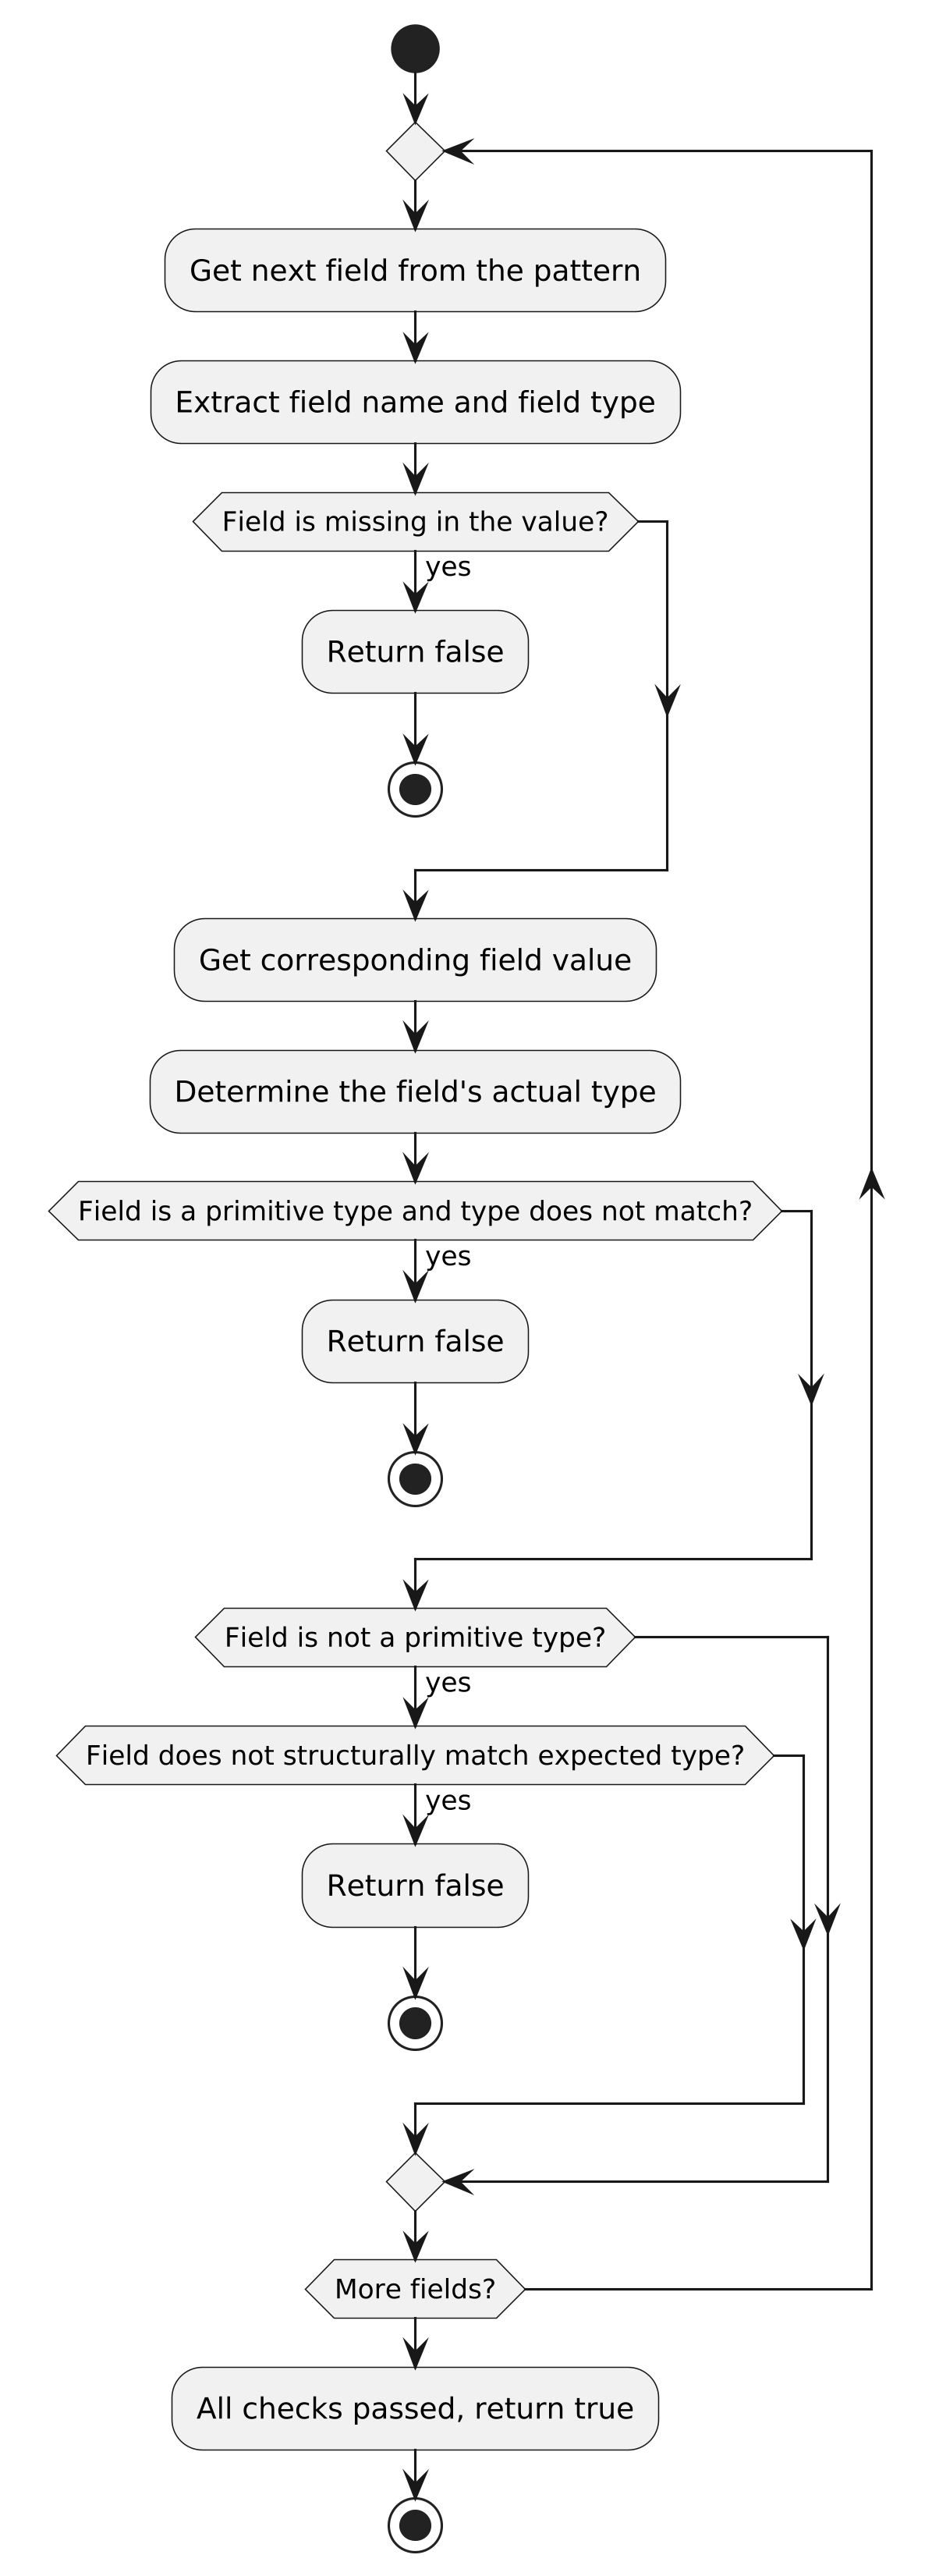
\includegraphics[scale=0.20]{./pics/matches_fields}}{}
	\caption{Matches operator property comparison.}
	\label{fig:implementation:matchesproperty}
\end{figure}

\begin{figure}[tb]
	\centering
	\def\stackalignment{r}
	\stackunder{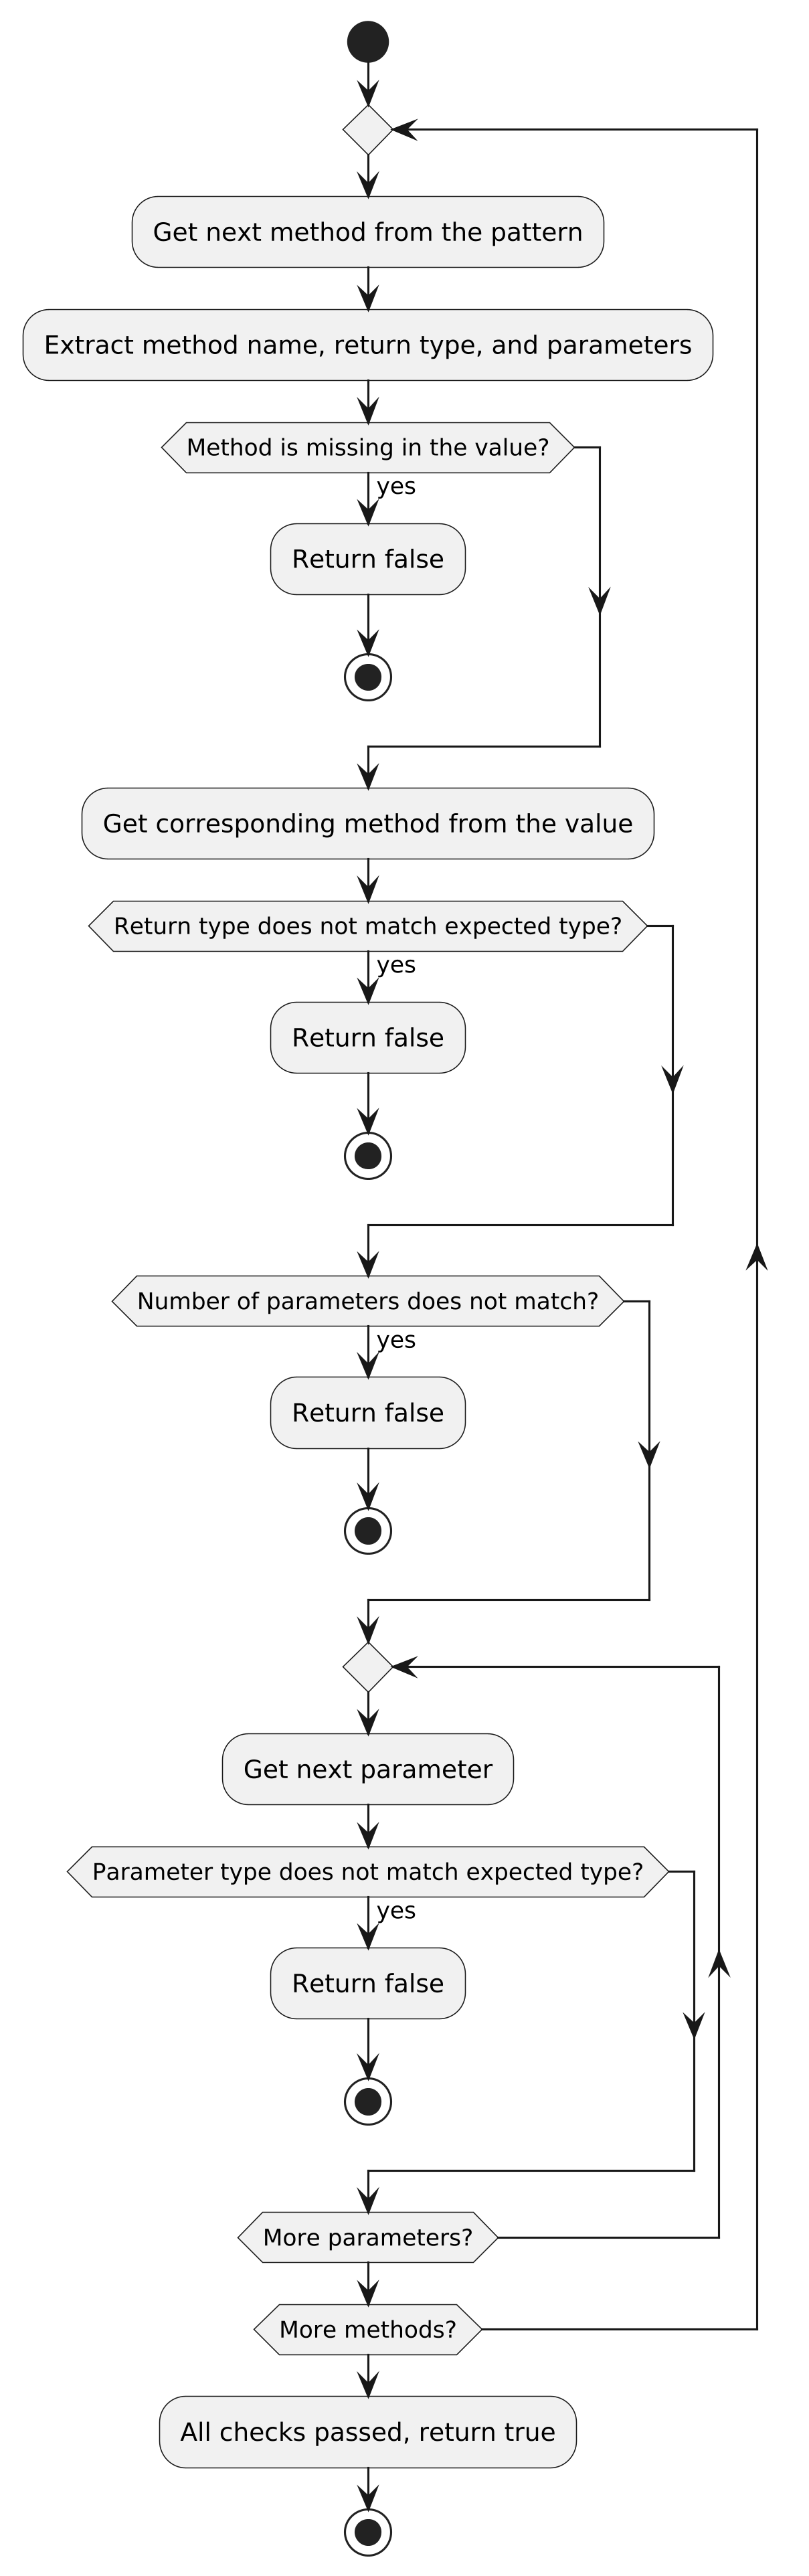
\includegraphics[scale=0.18]{./pics/matches_methods}}{}
	\caption{Matches operator method comparison.}
	\label{fig:implementation:matchesmethod}
\end{figure}

After verifying the properties, the matches expression iterates over the methods, as illustrated in Figure~\ref{fig:implementation:matchesmethod}. The process begins by searching for the method name within the target type. If a match is found, the return type is compared. Subsequently, each argument is examined by name, ensuring that the method signatures are identical. Additionally, the number of parameters is compared to enforce exact correspondence.

If none of these conditions evaluate to false, the input object is deemed compatible with the input type.

\subsection{Typeof Operator}
\label{sec:typeof}

In the Kipper programming language, the \lstinline|typeof| operator is used to obtain the type of an object at runtime. This operator can be used to check whether a variable or expression is of a particular type, such as a string, number, boolean, etc. It is most commonly used to check for \lstinline|null| and \lstinline|undefined| objects, in order to avoid type errors when the type of an object is unknown. The returned type object can be compared by reference to check for type equality. As shown in Listing~\ref{lst:implementation:typeofoperator}, the parentheses are optional. Both syntax styles are supported to align with Kipper's design goal of being similar to TypeScript and JavaScript, which implement it in the same way.

\begin{lstlisting}[language=Kipper,caption=Typeof operator used to determine the type of an input expression,label=lst:implementation:typeofoperator]
typeof 49; // "__kipper.builtIn.num"
typeof("Hello, World!"); // "__kipper.builtIn.str"
\end{lstlisting}

The \lstinline|typeof| operator in Kipper mirrors the functionality of TypeScript and JavaScript, but with enhancements tailored to Kipper's type system. Unlike JavaScript, where \lstinline|typeof null| returns \lstinline|object| due to historical reasons, Kipper correctly identifies \lstinline|null| as \lstinline|__kipper.builtIn.null|.

At runtime, the provided object is checked for its type using the target language's type features. A part of this process can be seen in Figure~\ref{fig:implementation:typeofimplementation}. The primitive types return their respective \lstinline|KipperRuntimeType|. Objects are a special case, as they can in JavaScript either be \lstinline|null|, an array, a class, or an object, such as one that implements an interface. The Figure is only a simplification of the algorithm and types like \lstinline|num| are hidden in order to display it in a compact way.

\begin{figure}[tb]
	\centering
	\def\stackalignment{r}
	\stackunder{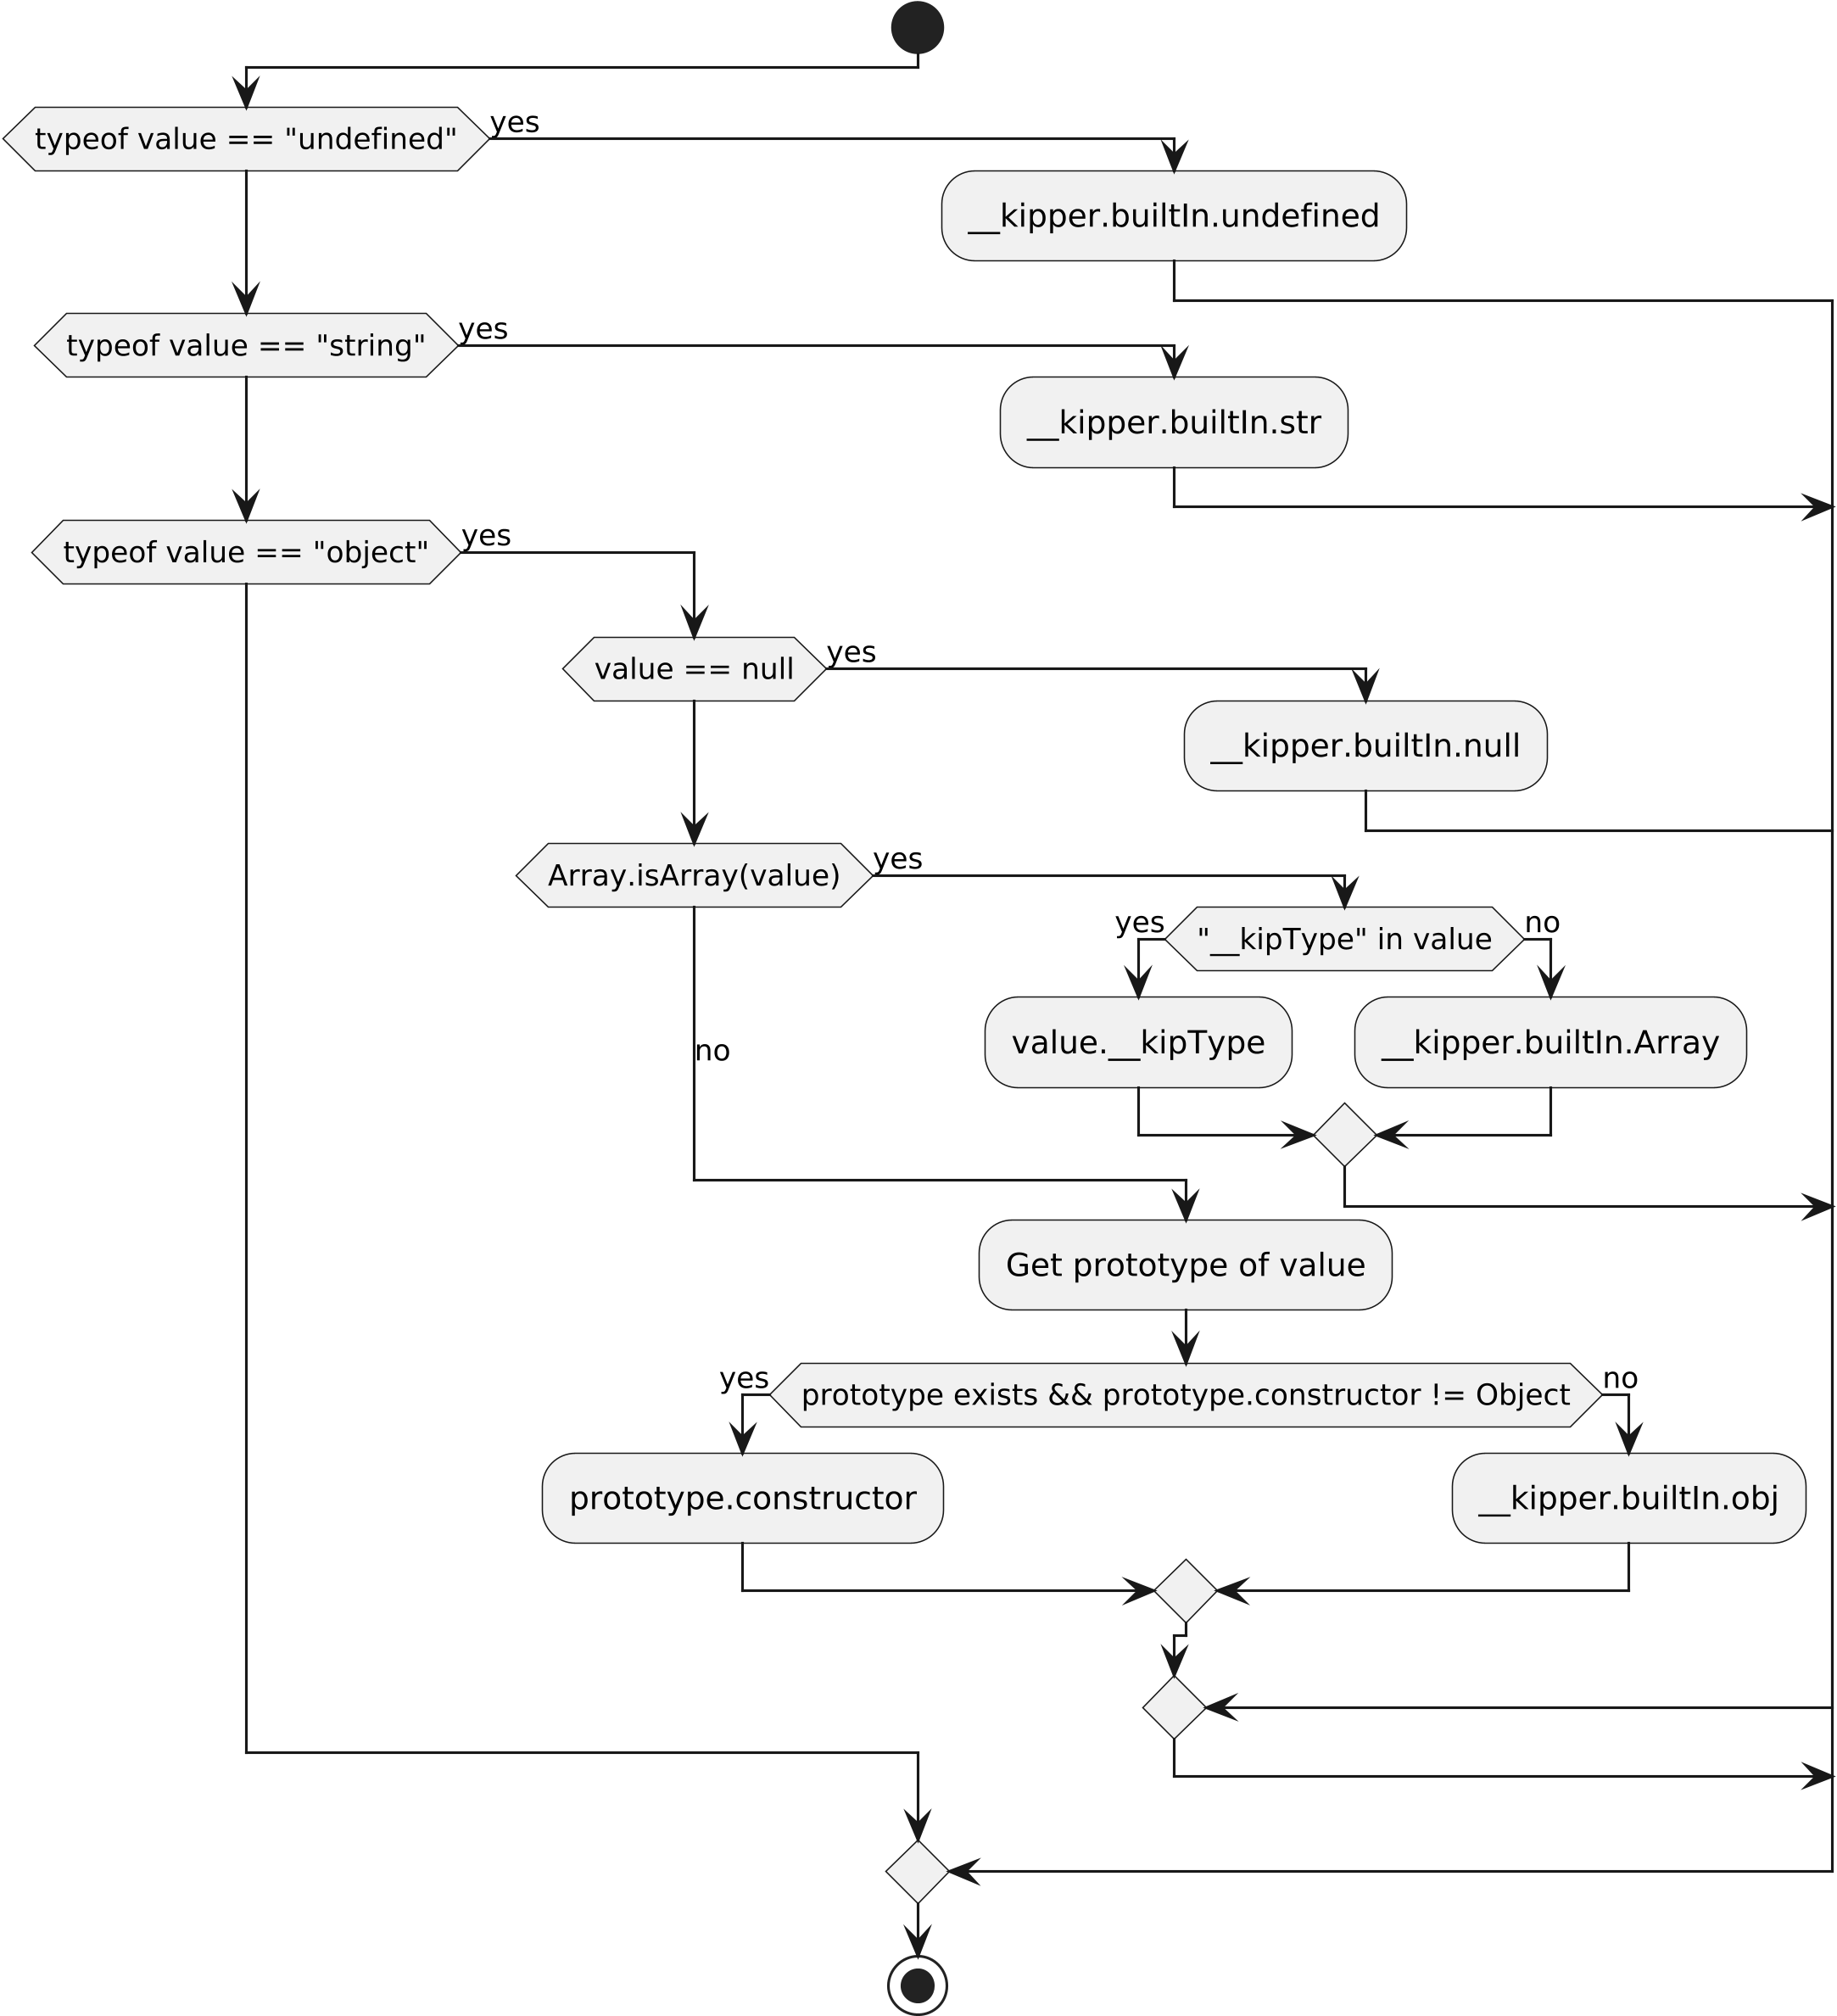
\includegraphics[scale=0.25]{./pics/typeOfImplementation}}{}
	\caption{Logical implementation of the \lstinline|typeof| operator in the target JavaScript/TypeScript environment. This is a simplified graph, which excludes certain basic types.}
	\label{fig:implementation:typeofimplementation}
\end{figure}

Although syntactically similar, the \lstinline|typeof| operator in the type declaration of a variable operates fundamentally differently, as demonstrated in Listing~\ref{lst:implementation:typeoftypespecifier}. This operator is referred to as \lstinline|TypeOfTypeSpecifier| and evaluates the type of a variable at compile time.

\begin{lstlisting}[language=Kipper,caption=Specifying the type based on a reference variable, label=lst:implementation:typeoftypespecifier]
var t: num = 3;
var count: typeof(t) = 4;
\end{lstlisting}

%%% Local Variables:
%%% mode: LaTeX
%%% TeX-master: "../thesis"
%%% End:
